\chapter{Verification and Results} \label{chap:ch4}

\section{Verification Methodology}\label{sec:verification_methodology}

Following the general \ac{IC} design flow described in Section~\ref{sec:ic_design_methodology}, this section outlines the specific tools and verification methodology adopted for the schematic design, layout implementation, and electrical validation of the transmitter driver presented in this dissertation.

Both the schematic design and the physical layout of the driver were carried out using Synopsys Custom Compiler. The design targets the GlobalFoundries 55\,nm LPx \ac{CMOS} technology, with device models, design rules, and electrical constraints obtained from the corresponding foundry-provided \ac{PDK} and \ac{DRM}.

\begin{figure}[H]
	\centering
	\resizebox{1\textwidth}{!}{
	\begin{tikzpicture}[transform shape]
		% Paths, nodes and wires:
		\node[shape=rectangle, draw, line width=1pt, minimum width=5.965cm, minimum height=9.965cm] at (10.75, 5){};
		\draw[line width=1pt] (8.75, 9) -- (8.75, 7) -- (10.75, 8) -- cycle node[anchor=center] at (9.75, 8){$PRE$};
		\draw (9.75, 8.5) to[short, *-, /tikz/circuitikz/bipoles/length=2.81cm] (12.75, 8.5);
		\draw[line width=1pt] (8.75, 6) -- (8.75, 4) -- (10.75, 5) -- cycle node[anchor=center] at (9.75, 5){$MAIN$};
		\draw (9.75, 5.5) to[short, *-, /tikz/circuitikz/bipoles/length=2.81cm, l={$TXn$}, label distance=-0.03cm] (14.75, 5.5);
		\draw (9.75, 4.5) to[short, /tikz/circuitikz/bipoles/length=2.81cm, l_={$TXp$}] (14.75, 4.5);
		\draw[line width=1pt] (8.75, 3) -- (8.75, 1) -- (10.75, 2) -- cycle node[anchor=center] at (9.75, 2){$POST$};
		\draw (9.75, 2.5) to[short, *-, /tikz/circuitikz/bipoles/length=2.81cm] (12.75, 2.5);
		\draw (9.75, 7.5) to[short] (11.75, 7.5);
		\draw (11.75, 7.5) to[short, -*, /tikz/circuitikz/bipoles/length=2.53cm] (11.75, 5.5);
		\draw (11.75, 5.5) |- (9.75, 1.5);
		\draw (12.75, 4.5) to[short, *-, /tikz/circuitikz/bipoles/length=2.53cm] (12.75, 8.5);
		\draw (12.75, 2.5) -| (12.75, 4.5);
		\draw (8.75, 8.5) -| (0.75, 8.5);
		\draw (8.75, 7.5) -| (0.75, 7.5);
		\draw (8.75, 4.5) |- (5.75, 4.5);
		\draw (8.75, 5.5) -- (5.75, 5.5);
		\draw (8.75, 2.5) -- (5.75, 2.5);
		\draw (8.75, 1.5) -- (5.75, 1.5);
		\node[shape=rectangle, draw, line width=1pt, minimum width=1.715cm, minimum height=1.465cm] at (4.875, 5){} node[anchor=center, align=center, text width=1.327cm, inner sep=6pt] at (4.875, 5){\Large 1UI};
		\draw (4.5, 8.5) to[short, *-] (4.5, 5.75);
		\draw (5.25, 8.5) to[short, *-] (5.25, 5.75);
		\node[shape=rectangle, draw, line width=1pt, minimum width=1.715cm, minimum height=1.465cm] at (4.875, 2){} node[anchor=center, align=center, text width=1.327cm, inner sep=6pt] at (4.875, 2){\Large 1UI};
		\draw (4.5, 4.25) -| (4.5, 2.75);
		\draw (5.25, 4.25) -| (5.25, 2.75);
		\draw (18.5, 1.75) to[empty diode] (18.5, 5.5);
		\draw (18.5, 5.5) to[short, *-] (16.25, 5.5);
		\draw (18.5, 5.5) to[empty diode] (18.5, 9);
		\draw (15.25, 3.75) to[capacitor, /tikz/circuitikz/bipoles/length=1.05cm, l_={$115 fF$}] (15.25, 2.75);
		\draw (16.25, 2.5) to[capacitor, /tikz/circuitikz/bipoles/length=1.05cm, l_={$115 fF$}] (16.25, 4);
		\draw (20.5, 5.5) to[capacitor, /tikz/circuitikz/bipoles/length=1.05cm, l={$265 nF$}] (22, 5.5);
		\draw (20.5, 4.5) to[capacitor, /tikz/circuitikz/bipoles/length=1.05cm, l_={$265 nF$}] (22, 4.5);
		\draw (16.25, 4) to[short, -*] (16.25, 5.5);
		\draw (15.25, 3.75) to[short, -*] (15.25, 4.5);
		\draw (19.75, 2.75) to[empty diode] (19.75, 4.5);
		\draw (19.75, 5.75) to[empty diode] (19.75, 8.75);
		\draw (18.5, 5.5) -- (20.5, 5.5);
		\draw (19.75, 5.75) to[short, -*] (19.75, 4.5);
		\draw (19.75, 2.75) -| (19.75, 1.75);
		\draw (16.25, 2.5) -| (16.25, 1.75);
		\draw (15.25, 2.75) -| (15.25, 1.75);
		\draw (19.75, 8.75) -| (19.75, 9);
		\node[shape=rectangle, draw, line width=1.9pt, dash pattern={on 7.6pt off 7.6pt}, minimum width=3.933cm, minimum height=9.933cm] at (4.75, 5){};
		\node[shape=rectangle, draw, line width=1pt, minimum width=5.965cm, minimum height=1.965cm] at (10.75, 12){} node[anchor=center, align=center, text width=5.577cm, inner sep=6pt] at (10.75, 12){\LARGE Control\\Block};
		\draw[line width=1.2pt] (8.5, 11) -- (8.5, 10);
		\draw[line width=1.2pt] (9, 11) -- (9, 10);
		\draw[line width=1.2pt] (11.25, 11) -- (11.25, 10);
		\draw[line width=1.2pt] (11.75, 11) -- (11.75, 10);
		\draw[line width=1.2pt] (12.25, 11) -- (12.25, 10);
		\node[shape=rectangle, draw, line width=1pt, minimum width=1.465cm, minimum height=1.965cm] at (22.75, 5){} node[anchor=center, align=center, text width=1.077cm, inner sep=6pt] at (22.75, 5){\LARGE s4p};
		\draw (23.5, 5.5) -- (24.75, 5.5);
		\draw (23.5, 4.5) -- (24.75, 4.5);
		\draw (24.75, 8) to[american resistor, /tikz/circuitikz/bipoles/length=1.05cm, l_={$50 \Omega$}] (24.75, 5.5);
		\draw (25.75, 8) to[american resistor, /tikz/circuitikz/bipoles/length=1.05cm, l={$50 \Omega$}] (25.75, 5.5);
		\draw (25.75, 5.5) -| (25.75, 4.5) -- (24.75, 4.5);
		\draw (24.75, 9) -| (24.75, 8);
		\draw (25.75, 9) -| (25.75, 8);
		\draw[line width=2.2pt] (18, 9) -- (20.25, 9);
		\draw[line width=2.2pt] (24.25, 9) -- (26.25, 9);
		\node[tlground, xscale=1.28, yscale=1.28] at (18.5, 1.25){};
		\node[tlground, xscale=1.28, yscale=1.28] at (19.75, 1.25){};
		\draw (18.5, 1.75) -| (18.5, 1.25);
		\draw (19.75, 1.75) -| (19.75, 1.25);
		\node[tlground, xscale=1.28, yscale=1.28] at (16.25, 1.25){};
		\node[tlground, xscale=1.28, yscale=1.28] at (15.25, 1.25){};
		\draw (15.25, 1.75) -| (15.25, 1.25);
		\draw (16.25, 1.75) -| (16.25, 1.25);
		\draw (16.25, 5.5) -- (14.75, 5.5);
		\draw (14.75, 4.5) -- (20.5, 4.5);
		\node[shape=rectangle, minimum width=1.465cm, minimum height=0.715cm] at (0.75, 8.875){} node[anchor=north west, align=left, text width=1.077cm, inner sep=6pt] at (-0, 9.25){DATAn};
		\node[shape=rectangle, minimum width=1.465cm, minimum height=0.715cm] at (0.75, 7.125){} node[anchor=north west, align=left, text width=1.077cm, inner sep=6pt] at (-0, 7.5){DATAp};
	\end{tikzpicture}
	}
	\caption{Driver testbench schematic}\label{fig:driver_testbench}
\end{figure}

Figure~\ref{fig:driver_testbench} shows the schematic of the testbench used to verify the \ac{TX} driver.

The taps are configured through a dedicated control block, implemented as a VerilogA logic module that generates the corresponding enable signals for each tap according to the desired settings. 

The differential input data, DATAp and DATAn, is generated by a bit-pattern generator with 15~ps rise and fall times, with DATAn produced as the complement of DATAp. A logic `0' bit is represented by a voltage level $V_{low} = V_{cm} - \Delta$, and a logic `1' bit by $V_{high} = V_{cm} + \Delta$, where $V_{cm}$ and $\Delta$ are defined as in the previous chapter, with $V_{cm} = 0.8$~V and $\Delta = 0.2$~V. The main-cursor and post-cursor tap inputs are obtained by delaying the pre-tap data using delay elements provided by the analoglib library, each configured for a delay of 1~\ac{UI}, corresponding to 100~ps at the target data rate. 

At the driver output, each of the TXp and TXn nodes is loaded with a 115~fF capacitor, and is additionally protected by a double-diode \ac{ESD} structure provided by the \ac{PDK}. Both output lines are \ac{AC}-coupled through 265~nF capacitors, as specified by the \ac{USB} 3.2 Gen~2 standard. 

The transmission channel itself is modeled as a four-port S-parameter block, implemented using the corresponding analoglib component and populated with an s4p file supplied by the \ac{USB-IF}, allowing the channel losses and reflections present in a real \ac{USB} 3.2 SuperSpeed link to be reproduced in simulation. At the channel output, two 50~$\Omega$ resistors are connected to emulate the termination presented by the \ac{RX}. 

Rise and fall times, output swing and output impedance are all measured with the channel model disconnected, so as to isolate these metrics from channel-induced distortion, while eye-diagram measurements are performed with the channel model connected, in order to capture its and equalization impact on the transmitted signal.

The verification methodology followed a two-stage evaluation process, consistent with the schematic-to-layout design flow described in Section~\ref{sec:ic_design_methodology}. In the first stage, pre-extraction results, obtained directly from schematic-level simulation without the inclusion of layout-induced parasitics, were evaluated against the normative \ac{USB} 3.2 specifications summarized in Section~\ref{sec:usb32_specs}, across the relevant \ac{PVT} corners, \ac{TT}, \ac{SS} and \ac{FF}, as well as across resistor corners accounting for variation in the poly and diffusion resistor models used within the design. This stage served to validate the functional correctness and nominal performance of the design prior to layout.

In the second stage, following the completion of the physical layout and parasitic extraction, the post-extraction results were compared with the corresponding pre-extraction results in order to quantify the performance changes introduced by layout parasitics. The extracted implementation was also evaluated against the same relevant \ac{USB} 3.2 numerical electrical limits and \ac{PVT} and resistor-corner sweeps used in the pre-extraction stage. This allowed the implemented driver to be assessed against the selected standard requirements once layout-induced effects were taken into account. Any target not met at this stage was addressed through iterative refinement of the layout and, where necessary, the schematic, consistent with the design flow described in Section~\ref{sec:ic_design_methodology}.

%\subsection{Simulation Setup and Test Conditions}
%    \paragraph{Testbenches for dc, tran, ac etc.}
\section{Driver Performance}

The normative output swing specification is measured with the system operating without equalization, i.e., with the driver configured in the EQ0 preset. For the tap enable mapping defined in Section~\ref{sec:eq_presets_current}, the 120 enabled current mirrors for the main tap were not enough to keep to swing within the normative range for all three \ac{PVT} corners, with an output swing of 0.677 V for the \ac{SS} corner, as shown in Figure~\ref{fig:PVT_vo_swing_main_120}. 

\begin{figure}[H]
  \includegraphics[width=0.9\textwidth]{chapter4/pre_ext/Vo_swing/PVT_PRE_0_MAIN_120_POST_0.png}
  \caption{Starting EQ0 output differential voltage for all three \ac{PVT} corners}\label{fig:PVT_vo_swing_main_120}
\end{figure}

This raised the need to add more units to the main tap in order to achieve the required swing range, which was done by adding four more units to the main tap, resulting in a total of 144 enabled current mirrors. The output swing for all three \ac{PVT} corners with the modified main tap is shown in Figure~\ref{fig:PVT_vo_swing_main_144}, where it can be seen that the output swing is now within the normative range for \ac{SS} and \ac{TT}, and slightly above the normative range for \ac{FF}, at 1.3 V, which is acceptable since it can be lowered by deactivating some of the current mirrors.

\begin{figure}[H]
  \includegraphics[width=0.8\textwidth]{chapter4/pre_ext/Vo_swing/PVT_PRE_0_MAIN_144_POST_0.png}
  \caption{Modified EQ0 output differential voltage for all three \ac{PVT} corners}\label{fig:PVT_vo_swing_main_144}
\end{figure}

This difference between the calculated and simulated output swing values can be attributed to the fact that the calculations in Section~\ref{sec:eq_presets_current} were based on idealized assumptions, such as perfect current mirror matching, which do not hold in practice, and can change the effective equalization performed by the driver. Table~\ref{tab:PVT_eq_results} summarizes the \ac{PS} and \ac{DE} values obtained for each equalization preset across the three simulated \ac{PVT} corners, and shows the difference between the simulated and target values. 

\begin{table}[htbp]
    \centering
    \caption{Equalization results across \ac{PVT} corners, expressed as \% deviation from target}
    \label{tab:PVT_eq_results_deviation}
    \begin{tabular}{lcccccc}
        \hline \hline
        \textbf{Preset} & \multicolumn{2}{c}{\textbf{TT}} & \multicolumn{2}{c}{\textbf{FF}} & \multicolumn{2}{c}{\textbf{SS}} \\
         & \textbf{PS} & \textbf{DE} & \textbf{PS} & \textbf{DE} & \textbf{PS} & \textbf{DE} \\
        \hline
        EQ1 & +8.33\% & -10\% & +4.17\% & -9.52\% & +20\% & -12.38\% \\
        EQ2 & -4.09\% & -7.74\% & -5.91\% & -9.68\% & +2.27\% & -6.77\% \\
        EQ3 & -5.94\% & -5.29\% & -6.56\% & -6.29\% & -0.62\% & -3\% \\
        EQ4 & +0.4\% & -7.4\% & -1.6\% & -8.2\% & +6.4\% & -4.6\% \\
        \hline \hline
    \end{tabular}
\end{table}


\begin{center}
\captionof{table}{Equalization results for \ac{PVT} corners}\label{tab:PVT_eq_results}
\begin{tabular}{cccccccc}
  \hline \hline
  \textbf{Preset} & \textbf{Process} & \textbf{VDD} & \textbf{Temp} & \textbf{PS} & \textbf{DE} & \textbf{Target PS} & \textbf{Target DE} \\
  \hline 
  EQ1 & TT & 1.2 & 25 & 1.30 & 1.89 & 1.2 & 2.1\\
  EQ1 & FF & 1.26 & -40 & 1.25 & 1.90 & 1.2 & 2.1\\
  EQ1 & SS & 1.14 & 125 & 1.44 & 1.84 & 1.2 & 2.1\\

  EQ2 & TT & 1.2 & 25 & 2.11 & 2.86 & 2.2 & 3.1\\
  EQ2 & FF & 1.26 & -40 & 2.07 & 2.80 & 2.2 & 3.1\\
  EQ2 & SS & 1.14 & 125 & 2.25 & 2.89 & 2.2 & 3.1\\

  EQ3 & TT & 1.2 & 25 & 3.01 & 6.63 & 3.2 & 7\\
  EQ3 & FF & 1.26 & -40 & 2.99 & 6.56 & 3.2 & 7\\
  EQ3 & SS & 1.14 & 125 & 3.18 & 6.79 & 3.2 & 7\\

  EQ4 & TT & 1.2 & 25 & 2.51 & 4.63 & 2.5 & 5\\
  EQ4 & FF & 1.26 & -40 & 2.46 & 4.59 & 2.5 & 5\\
  EQ4 & SS & 1.14 & 125 & 2.66 & 4.77 & 2.5 & 5\\
  \hline \hline
\end{tabular}
\end{center}

Figure~\ref{fig:tap_iss_sweep} shows the sweep of each tap $I_{SS}$ for their enable signals, where it can be seen that the current sunk suffer from slight variations with the increase of enabled current mirrors. These current variations adds up and results in the differences between the calculated and simulated \ac{PS} and \ac{DE} values shown in Table~\ref{tab:PVT_eq_results}. 
The table shoes that EQ1 does not meet the normative equalization range. This can be improved by adjusting the number of enabled current mirrors, as shown further in Section~\ref{sec:pext_results}.

\begin{figure}[H]
	\begin{subfigure}[b]{0.4\textwidth}
		\centering
		\resizebox{\linewidth}{!}{
		\begin{tikzpicture}
			\begin{axis}[
				xlabel={en},
				ylabel={$I_{SS}$ (mA)},  
				minor tick num=1, 
				grid=both,
				legend pos=south east,
        no markers,
        every axis plot/.append style={line width=1.2pt},
			]
				\addplot table [blue, col sep=comma, x=en, y=iss] {plot/Iss_PRE_en_sweep.csv};
			\end{axis}
		\end{tikzpicture}
		}
		\caption{Pre tap}\label{fig:pre_tap_iss}
	\end{subfigure}
	\begin{subfigure}[b]{0.4\textwidth}
		\centering
		\resizebox{\linewidth}{!}{
		\begin{tikzpicture}
			\begin{axis}[
				xlabel={en},
				ylabel={$I_{SS}$ (mA)},  
				minor tick num=1, 
				grid=both,
        no markers,
        every axis plot/.append style={line width=1.2pt},
			]
				\addplot table [blue, col sep=comma, x=en, y=iss] {plot/Iss_POST_en_sweep.csv};
			\end{axis}
		\end{tikzpicture}
		}
		\caption{Post tap}\label{fig:post_tap_iss}
	\end{subfigure}
	\begin{subfigure}{0.4\textwidth}
		\centering
		\resizebox{\linewidth}{!}{
		\begin{tikzpicture}
			\begin{axis}[
				xlabel={en},
				ylabel={$I_{SS}$ (mA)},  
				minor tick num=1, 
				grid=both,
				legend pos=south east,
        no markers,
        every axis plot/.append style={line width=1.2pt},
			]
				\addplot table [blue, col sep=comma, x=en, y=iss] {plot/Iss_MAIN_en_sweep.csv};
			\end{axis}
		\end{tikzpicture}
		}
		\caption{Main tap}\label{fig:main_tap_iss}
	\end{subfigure}
	\caption{Sweep of each tap $I_{SS}$ for their enable signals}\label{fig:tap_iss_sweep}
\end{figure}

\subsection{Output Impedance Across PVT and Resistor Corners} \label{sec:zout_pvt_corners}

In addition to the standard \ac{PVT} corners considered in the verification methodology described in Section~\ref{sec:verification_methodology}, the use of technology-provided polysilicon resistances for the termination network, discussed in Section~\ref{sec:overall_driver_architecture}, introduces an additional set of corners associated with the resistor process variation itself: a minimum resistance corner (Res\_min), a nominal resistance corner (Res\_nom), and a maximum resistance corner (Res\_max). Since these resistor corners are, in principle, independent of the standard PVT corners, they must be analyzed jointly with the PVT corners rather than in isolation, in order to correctly capture the full range of expected output impedance variation.

The differential output impedance of the driver is particularly sensitive to these resistor corners, since the termination network is composed entirely of passive resistors, as described in Section~\ref{sec:overall_driver_architecture}, and its resistance therefore varies directly with the underlying resistor process corner, independently of the transistor-level \ac{PVT} corner.

Figure~\ref{fig:zout_PVT} shows the resulting differential output impedance across the combined \ac{PVT} and resistor corner space, as a function of the number of termination bank resistors activated, ranging from 0 to the full 32 resistors available. The results for each \ac{PVT} process corner are shown in Figure~\ref{fig:zout_PVT}.

Across all evaluated \ac{PVT} corners, the differential output impedance remains within the normative range of 72\,$\Omega$ to 120\,$\Omega$ specified by the \ac{USB} 3.2 Gen~2 standard, discussed in Section~\ref{sec:usb32_specs}, confirming that the termination bank provides sufficient tuning range and resolution to maintain compliant impedance matching under the combined effect of \ac{PVT} and resistor process variation.

\begin{figure}[H]
  \centering
	\begin{subfigure}{0.4\textwidth}
		\centering
		\includegraphics[width=\linewidth]{chapter4/pre_ext/Zout/TT.png}
		\caption{\ac{TT}}\label{fig:zout_TT_PVT}
	\end{subfigure}
	\begin{subfigure}{0.4\textwidth}
		\centering
		\includegraphics[width=\linewidth]{chapter4/pre_ext/Zout/FF.png}
		\caption{\ac{FF}}\label{fig:zout_FF_PVT}
	\end{subfigure}
	\begin{subfigure}{0.4\textwidth}
		\centering
		\includegraphics[width=\linewidth]{chapter4/pre_ext/Zout/SS.png}
		\caption{\ac{SS}}\label{fig:zout_SS_PVT}
	\end{subfigure}
	\caption{Differential output impedance across corners and bank configurations}\label{fig:zout_PVT}
\end{figure}

Table~\ref{tab:zout_PVT} summarizes the number of termination bank resistors that must be enabled in order to achieve the maximum and minimum output impedance values across the combined \ac{PVT} and resistor corner space, as well as the corresponding number of resistors required to achieve the nominal differential impedance of 100\,$\Omega$. 

\begin{table}[H]
 \centering
 \caption{$\mathrm{Z_{out, diff}}$ across \ac{PVT} and resistor corners}
 \label{tab:zout_PVT}
 \begin{tabular}{ccccc}
  \hline
  \textbf{PVT} & \textbf{Res} & \textbf{\#$\mathrm{en_{max}}$} & \textbf{\#$\mathrm{en_{nom}}$} & \textbf{\#$\mathrm{en_{min}}$}\\
  \hline \hline
  TT & Res\_min & 3 & 8 & 18\\
  TT & Res\_nom & 9 & 15 & 28\\
  TT & Res\_max & 15 & 22 & NA\\
  SS & Res\_min & NA & NA & 6\\ % SS Rmin cai muito rápido
  SS & Res\_nom & NA & 1 & NA\\
  SS & Res\_max & 6 & 23 & NA\\
  FF & Res\_min & 4 & 7 & 15\\
  FF & Res\_nom & 6 & 10 & 20\\
  FF & Res\_max & 9 & 14 & 26\\
  \hline \hline
 \end{tabular}
\end{table}

\subsection{Signal Integrity}\label{sec:pre_SI}
% Duty Cycle Distortion por conta do rise time ser maior que o fall time  
% EYE DIAG - BIT PERIOD : HORIZONTAL WIDTH IS USED AS TIME REFERENCE TO MEASURE JITTER (https://www.protoexpress.com/blog/analyzing-eye-diagrams-for-signal-integrity-high-speed-pcbs/      https://www.protoexpress.com/blog/techniques-to-measure-and-avoid-jitter-in-pcbs/ )

Rise and fall time performance of the transmitter driver, discussed in the context of slew rate in Section~\ref{sec:slew_rate}, was characterized using the modified EQ0 preset, corresponding to the full main-tap configuration with all 144 main-tap current mirrors enabled and no pre-cursor or post-cursor equalization applied, driving a load capacitance of 115\,fF.

The pre-extraction rise and fall waveforms across the three \ac{PVT} corners are presented in Figure~\ref{fig:rise_fall_PVT}.

\begin{figure}[H]
  \centering
	\begin{subfigure}{0.32\textwidth}
		\centering
		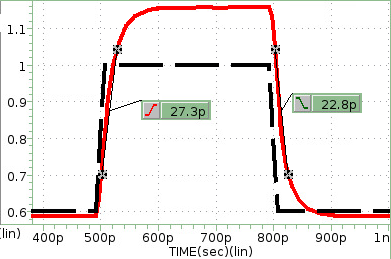
\includegraphics[width=\linewidth]{chapter4/pre_ext/rise_fall_times/TT.png}
		\caption{\ac{TT}}\label{fig:rise_fall_TT}
	\end{subfigure}
	\begin{subfigure}{0.32\textwidth}
		\centering
		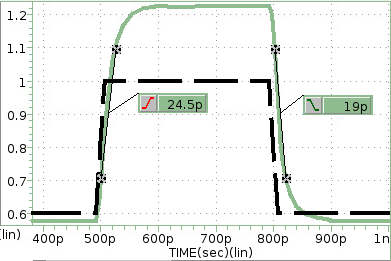
\includegraphics[width=\linewidth]{chapter4/pre_ext/rise_fall_times/FF.png}
		\caption{\ac{FF}}\label{fig:rise_fall_FF}
	\end{subfigure}
	\begin{subfigure}{0.32\textwidth}
		\centering
		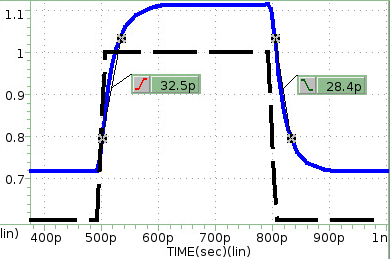
\includegraphics[width=\linewidth]{chapter4/pre_ext/rise_fall_times/SS.png}
		\caption{\ac{SS}}\label{fig:rise_fall_SS}
	\end{subfigure}
	\caption{Rise and fall times across \ac{PVT} corners}\label{fig:rise_fall_PVT}
\end{figure}

\begin{table}[htbp]
 \centering
 \caption{Rise and fall times across \ac{PVT} corners}
 \label{tab:rise_fall_PVT_pext}
 \begin{tabular}{ccc}
  \hline \hline
  \textbf{Corner} & \textbf{Rise} & \textbf{Fall} \\
  \hline
  TT & \SI{27.3}{\pico\second} & \SI{22.8}{\pico\second} \\
  FF & \SI{24.5}{\pico\second} & \SI{19}{\pico\second} \\
  SS & \SI{32.5}{\pico\second} & \SI{28.4}{\pico\second} \\
  \hline \hline
 \end{tabular}
\end{table}

Across all three corners, a consistent asymmetry is observed between the rise and fall times, with the fall time being shorter than the rise time in every case. This asymmetry is a direct consequence of the \ac{CML} topology adopted for the driver, discussed in Section~\ref{sec:tx_driver_architectures}, which implements an actively switched \ac{PDN} together with a passive \ac{PUN}.

Despite this asymmetry, the rise and fall times remain well within the nominal \ac{UI} of 100\,ps across all evaluated \ac{PVT} corners, indicating that the driver retains sufficient timing margin for correct operation at the target 10\,Gb/s data rate.

The channel model used to evaluate the transmitted and received eye diagrams is provided by the \ac{USB-IF}, and its insertion loss profile, $S_{21}$, is shown in Figure~\ref{fig:channel_S21}. The channel is supplied as a Touchstone file, named \texttt{Mock\_Host\_Cascaded\_Model\_TypeC\_rspl.s4p}, available at~\cite{usbif_channel_model}. This channel introduces an insertion loss of 21.6\,dB at 5\,GHz, corresponding to the Nyquist frequency of the 10\,Gb/s data rate. The input data source is a \ac{PRBS} \ac{LFSR} mode PN32, that generates the pseudo random bit sequence used to generate the transitions. A transient analysis was done for a runtime of 10000 $\times$ \ac{UI}, with a step of 10 ps.

\begin{figure}[H]
  \centering
  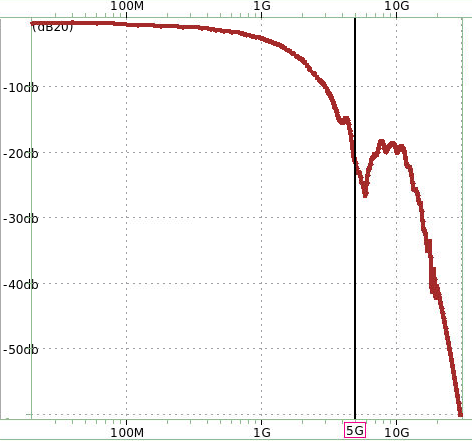
\includegraphics[width=0.5\linewidth]{chapter4/pre_ext/eyes/with_channel/channel_S21.png}
  \caption{Channel model $\mathrm{S_{21}}$}\label{fig:channel_S21}
\end{figure}

The following eye diagrams were obtained at the \ac{TT} and Res\_nom corner, for each of the five equalization presets defined in Section~\ref{sec:tx_equalization}. For each preset, both the \ac{TX} eye, measured directly at the driver output, and the \ac{RX} eye, measured after propagation through the reference channel, are evaluated. The corresponding metrics are summarized in Table~\ref{tab:rx_eye_pvt}.

The improvement of the received signal when transmitter equalization is applied can be clearly observed in the eye diagrams. The RX eye opening increases substantially from EQ0 through EQ3, demonstrating the effectiveness of the transmitter FFE in compensating for the reference-channel loss. The trend is not strictly monotonic for the strongest preset, however, since EQ4 produces a slightly smaller received eye than EQ3, indicating that EQ3 is the best preset for this particular channel model. The corresponding eye-diagram metrics are summarized in Table~\ref{tab:rx_eye_pvt}.

The results demonstrate a substantial improvement in received eye opening as transmitter equalization is increased from EQ0 toward EQ3. The trend is not strictly monotonic through EQ4, however, since the largest pre-extraction \ac{RX} eye is obtained with EQ3.

For EQ0, the \ac{TX} eye has a height of \SI{823}{\milli\volt} and a width of \SI{93.2}{\pico\second}, whereas the \ac{RX} eye is almost completely closed, with only \SI{3.35}{\milli\volt} of height and \SI{4.71}{\pico\second} of width. This confirms that the loss of the selected reference channel cannot be adequately compensated without transmitter equalization.

The corresponding unequalized \ac{TX} and \ac{RX} eye diagrams are presented in Figure~\ref{fig:eye_TT_EQ0}.

\begin{figure}[H]
  \centering
	\begin{subfigure}{0.49\textwidth}
		\centering
		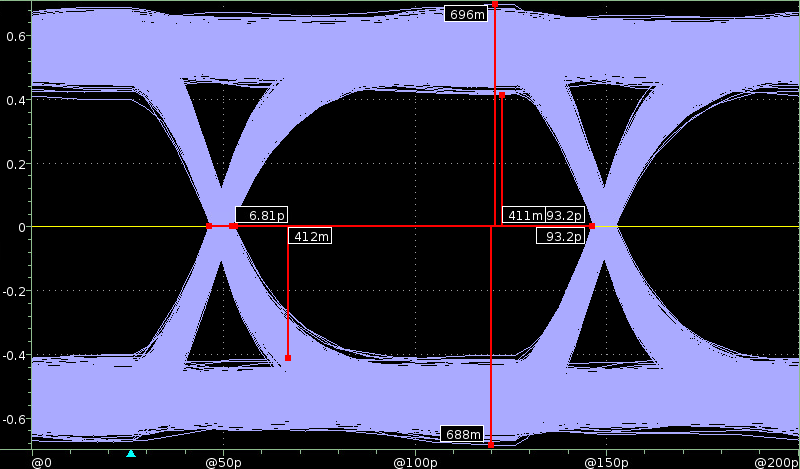
\includegraphics[width=\linewidth]{chapter4/pre_ext/eyes/with_channel/EQ0_TT_TX.png}
		\caption{\ac{TX}}\label{fig:eye_TT_EQ0_TX}
	\end{subfigure}
	\centering
	\begin{subfigure}{0.49\textwidth}
		\centering
		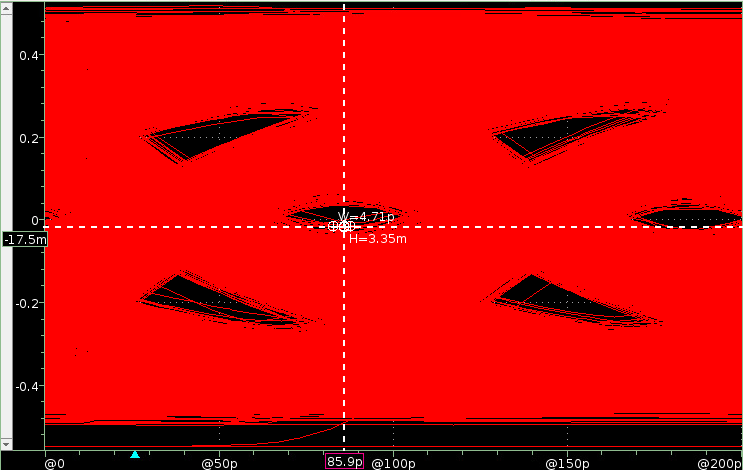
\includegraphics[width=\linewidth]{chapter4/pre_ext/eyes/with_channel/EQ0_TT_RX.png}
		\caption{\ac{RX}}\label{fig:eye_TT_EQ0_RX}
	\end{subfigure}
	\caption{Eye diagrams for EQ0 at corner \ac{TT}}\label{fig:eye_TT_EQ0}
\end{figure}

For EQ1, the \ac{RX} eye increases to \SI{132.1}{\milli\volt} in height and
\SI{54}{\pico\second} in width. EQ2 further increases the opening to
\SI{162}{\milli\volt} and \SI{60.2}{\pico\second}.

Figure~\ref{fig:eye_TT_EQ1} shows the \ac{TX} and \ac{RX} eye diagrams for the EQ1 preset.

\begin{figure}[H]
  \centering
	\begin{subfigure}{0.49\textwidth}
		\centering
		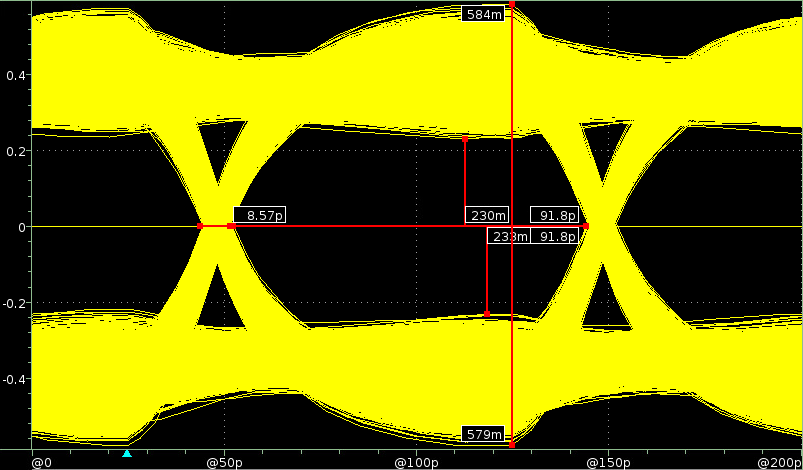
\includegraphics[width=\linewidth]{chapter4/pre_ext/eyes/with_channel/EQ1_TT_TX.png}
		\caption{\ac{TX}}\label{fig:eye_TT_EQ1_TX}
	\end{subfigure}
	\begin{subfigure}{0.49\textwidth}
		\centering
		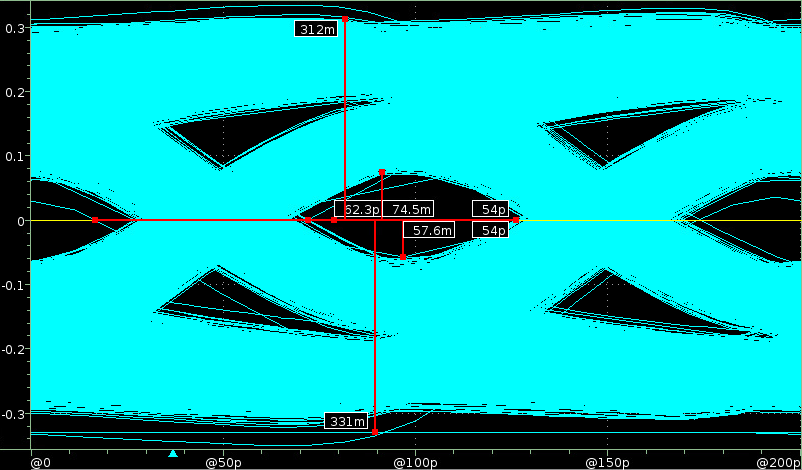
\includegraphics[width=\linewidth]{chapter4/pre_ext/eyes/with_channel/EQ1_TT_RX.png}
		\caption{\ac{RX}}\label{fig:eye_TT_EQ1_RX}
	\end{subfigure}
	\caption{Eye diagrams for EQ1 at corner \ac{TT}}\label{fig:eye_TT_EQ1}
\end{figure}

%For preset EQ2, shown in Figures~\ref{fig:eye_TT_EQ2_TX} and~\ref{fig:eye_TT_EQ2_RX}, the \ac{TX} eye has a height of 0.388\,V and a width of 90.5\,ps, while the \ac{RX} eye has a height of 0.186\,V and a width of 62\,ps. As with EQ1, the \ac{RX} eye height stays out of the keep-out region of the normative eye mask, but with vey little voltage margin.

Figure~\ref{fig:eye_TT_EQ2} shows the \ac{TX} and \ac{RX} eye diagrams for the EQ2 preset.

\begin{figure}[H]
  \centering
	\begin{subfigure}{0.49\textwidth}
		\centering
		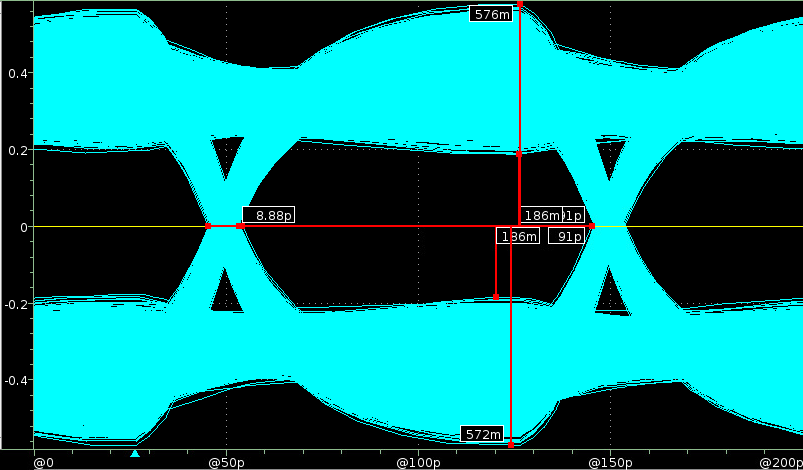
\includegraphics[width=\linewidth]{chapter4/pre_ext/eyes/with_channel/EQ2_TT_TX.png}
		\caption{\ac{TX}}\label{fig:eye_TT_EQ2_TX}
	\end{subfigure}
	\begin{subfigure}{0.49\textwidth}
		\centering
		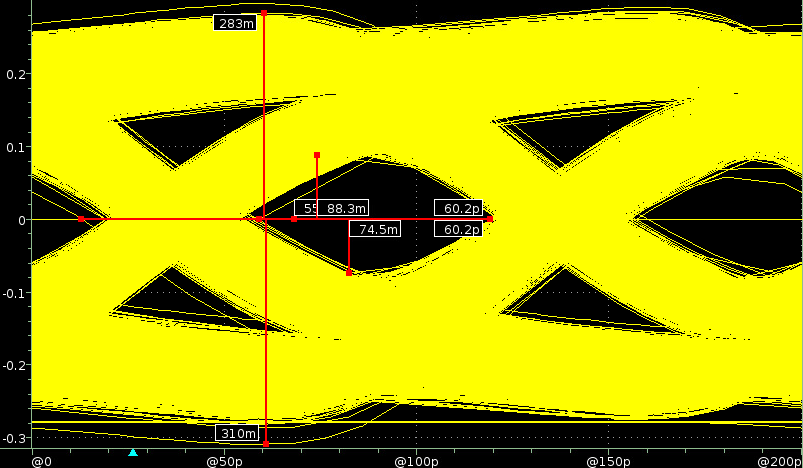
\includegraphics[width=\linewidth]{chapter4/pre_ext/eyes/with_channel/EQ2_TT_RX.png}
		\caption{\ac{RX}}\label{fig:eye_TT_EQ2_RX}
	\end{subfigure}
	\caption{Eye diagrams for EQ2 at corner \ac{TT}}\label{fig:eye_TT_EQ2}
\end{figure}

%For preset EQ3, shown in Figures~\ref{fig:eye_TT_EQ3_TX} and~\ref{fig:eye_TT_EQ3_RX}, the \ac{TX} eye has a height of 0.210\,V and a width of 88.7\,ps, while the \ac{RX} eye has a height of 0.253\,V and a width of 80.3\,ps. This setting results in the best eye at the \ac{RX} from all the evaluated equalization presets, with both the eye height and width falling well within the normative specification and with both good timing and voltage margin.

The largest pre-extraction eye is obtained with EQ3, which produces an \ac{RX} eye height of \SI{231}{\milli\volt} and a width of \SI{79.6}{\pico\second}. EQ4 also provides a widely open received eye, but its height of \SI{201.9}{\milli\volt} and width of \SI{73.1}{\pico\second} are both slightly smaller than those obtained with EQ3. EQ3 is therefore selected as the representative equalization preset for the subsequent pre-extraction corner analysis.

Figure~\ref{fig:eye_TT_EQ3} shows the \ac{TX} and \ac{RX} eye diagrams for EQ3, the preset yielding the largest pre-extraction received eye.

\begin{figure}[H]
  \centering
	\begin{subfigure}{0.49\textwidth}
		\centering
		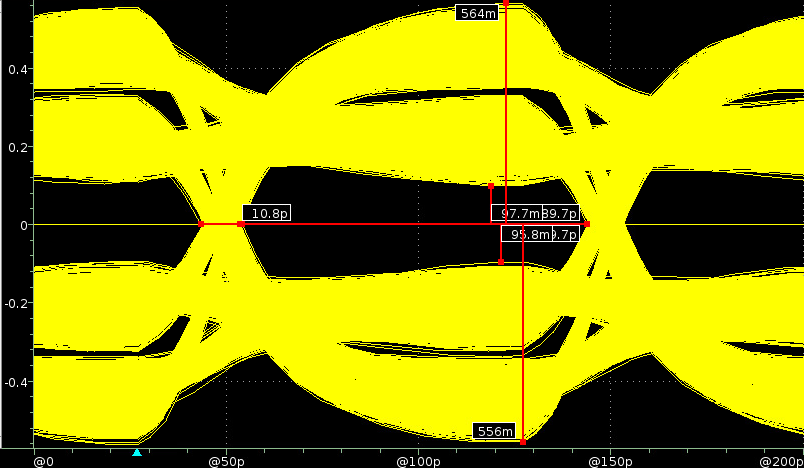
\includegraphics[width=\linewidth]{chapter4/pre_ext/eyes/with_channel/EQ3_TT_TX.png}
		\caption{\ac{TX}}\label{fig:eye_TT_EQ3_TX}
	\end{subfigure}
	\begin{subfigure}{0.49\textwidth}
		\centering
		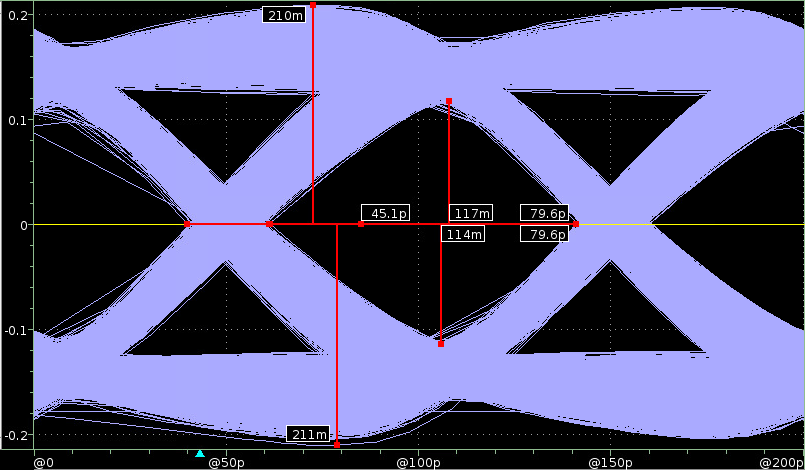
\includegraphics[width=\linewidth]{chapter4/pre_ext/eyes/with_channel/EQ3_TT_RX.png}
		\caption{\ac{RX}}\label{fig:eye_TT_EQ3_RX}
	\end{subfigure}
	\caption{Eye diagrams for EQ3 at corner \ac{TT}}\label{fig:eye_TT_EQ3}
\end{figure}

%For preset EQ4, shown in Figures~\ref{fig:eye_TT_EQ4_TX} and~\ref{fig:eye_TT_EQ4_RX}, the \ac{TX} eye has a height of 0.299\,V and a width of 89.6\,ps, while the \ac{RX} eye has a height of 0.226\,V and a width of 74\,ps. As with EQ3, this setting achieves the specification with some good margin.

Figure~\ref{fig:eye_TT_EQ4} shows the \ac{TX} and \ac{RX} eye diagrams for the stronger EQ4 preset.

\begin{figure}[H]
  \centering
	\begin{subfigure}{0.49\textwidth}
		\centering
		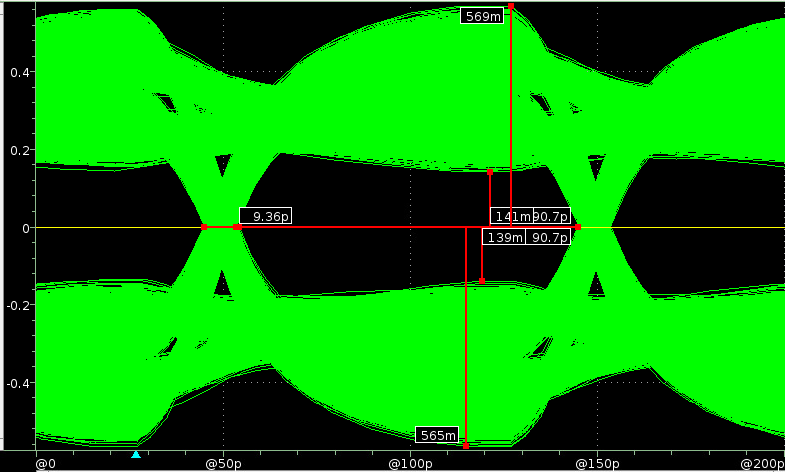
\includegraphics[width=\linewidth]{chapter4/pre_ext/eyes/with_channel/EQ4_TT_TX.png}
		\caption{\ac{TX}}\label{fig:eye_TT_EQ4_TX}
	\end{subfigure}
	\begin{subfigure}{0.49\textwidth}
		\centering
		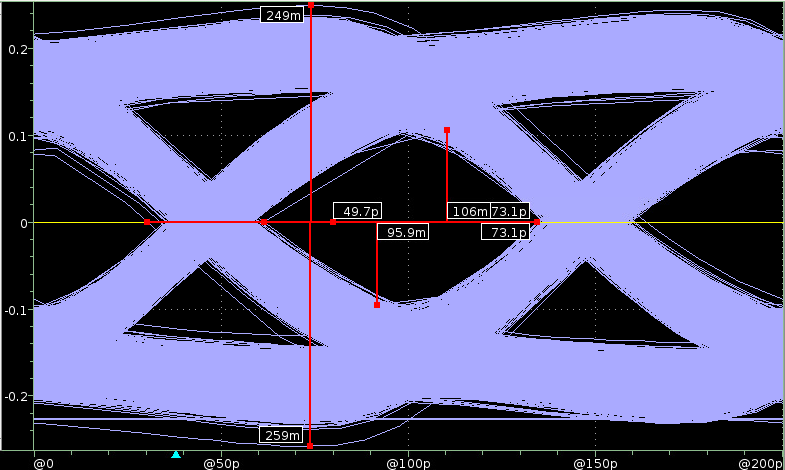
\includegraphics[width=\linewidth]{chapter4/pre_ext/eyes/with_channel/EQ4_TT_RX.png}
		\caption{\ac{RX}}\label{fig:eye_TT_EQ4_RX}
	\end{subfigure}
	\caption{Eye diagrams for EQ4 at corner \ac{TT}}\label{fig:eye_TT_EQ4}
\end{figure}

It should be noted that these preset coefficient values were used primarily as a general target during the design of the equalizer, rather than as an exact target to be matched precisely by the fabricated tap weights. 

\begin{table}[H]
 \centering
 \caption{\ac{TX} and \ac{RX} eye diagram metrics at \ac{TT} for different equalization presets}
 \label{tab:rx_eye_pvt}
 \begin{tabular}{ccccc}
  \hline \hline
   \textbf{EQ} 	  & \textbf{TX} 	   & \textbf{TX}    & \textbf{RX} 	& \textbf{RX} \\
   \textbf{Preset} & \textbf{Height} & \textbf{Width} & \textbf{Height} & \textbf{Width}\\
  \hline
  EQ0 & \SI{823}{\milli\volt} & \SI{93.2}{\pico\second} & \SI{3.35}{\milli\volt} & \SI{4.71}{\pico\second}\\
  EQ1 & \SI{463}{\milli\volt} & \SI{91.8}{\pico\second} 	& \SI{132.1}{\milli\volt} & \SI{54}{\pico\second}\\
  EQ2 & \SI{372}{\milli\volt} & \SI{91}{\pico\second} & \SI{162}{\milli\volt} & \SI{60.2}{\pico\second}\\
  EQ3 & \SI{193.5}{\milli\volt} & \SI{89.7}{\pico\second} & \SI{231}{\milli\volt} & \SI{79.6}{\pico\second}\\
  EQ4 & \SI{280}{\milli\volt} & \SI{90.7}{\pico\second} & \SI{201.9}{\milli\volt} & \SI{73.1}{\pico\second}\\
  \hline \hline
 \end{tabular}
\end{table}

The results presented above show that not all of the defined equalization presets are equally well suited to the specific channel used in this evaluation, with a considerable performance difference between EQ1 and EQ2 from EQ3 and EQ4. %This outcome, however, is attributable to the choice of equalization setting relative to the channel's loss profile, rather than to a limitation of the driver itself, and can be improved by appropriately tuning the driver's current mirror and termination bank settings to better match the equalization requirements of this specific channel, with no changes to the underlying driver design required to achieve this improvement. 
This outcome shows that, from the five defined equalization presets, EQ3 is the best suited to the specific channel used in this evaluation, producing the largest received eye opening and therefore the best \ac{SI} performance. For different channel loss profiles, however, the best equalization preset may differ from EQ3. 

To evaluate the impact of \ac{PVT} and resistor variation on the \ac{SI} of the transmitted signal, EQ3 was selected as the representative equalization preset, since it produces the largest \ac{RX} eye among the five pre-extraction configurations evaluated at \ac{TT}. The resulting \ac{RX} eye height and width for the \ac{TT}, \ac{FF}, and \ac{SS} process corners are reported in Tables~\ref{tab:eq3_eye_res_TT},~\ref{tab:eq3_eye_res_FF}, and~\ref{tab:eq3_eye_res_SS}, respectively.

The EQ3 received eye diagrams at \ac{TT} for the three resistor corners are compared in Figure~\ref{fig:eye_EQ3_TT}.

\begin{figure}[H]
  \centering
	\begin{subfigure}{0.49\textwidth}
		\centering
		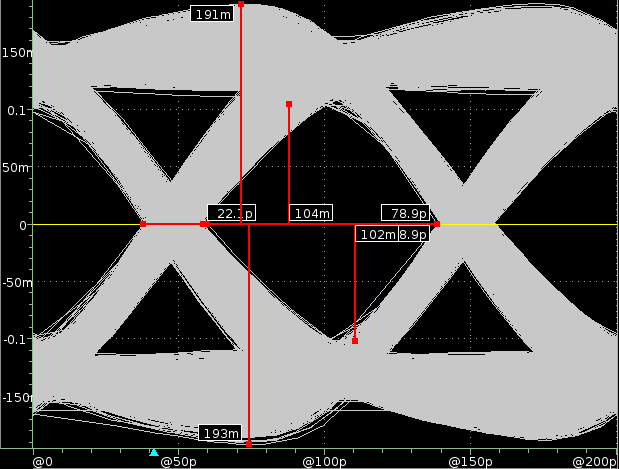
\includegraphics[width=\linewidth]{chapter4/pre_ext/eyes/with_channel/EQ3/EQ3_TT_Rmin.png}
		\caption{Res\_min}\label{fig:eye_EQ3_TT_Rmin}
	\end{subfigure}
	\begin{subfigure}{0.49\textwidth}
		\centering
		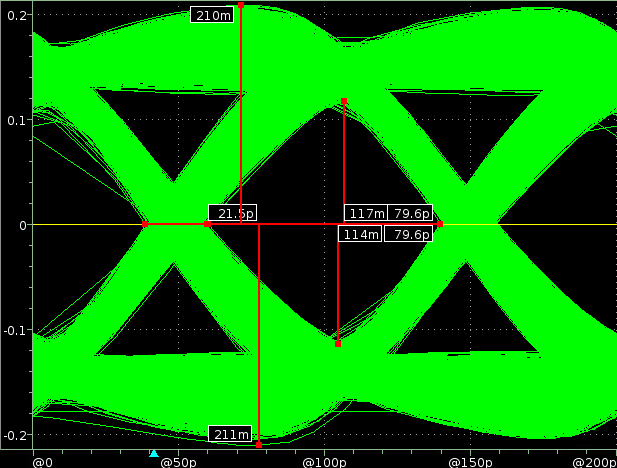
\includegraphics[width=\linewidth]{chapter4/pre_ext/eyes/with_channel/EQ3/EQ3_TT_Rnom.png}
		\caption{Res\_nom}\label{fig:eye_EQ3_TT_Rnom}
	\end{subfigure}
	\begin{subfigure}{0.49\textwidth}
		\centering
		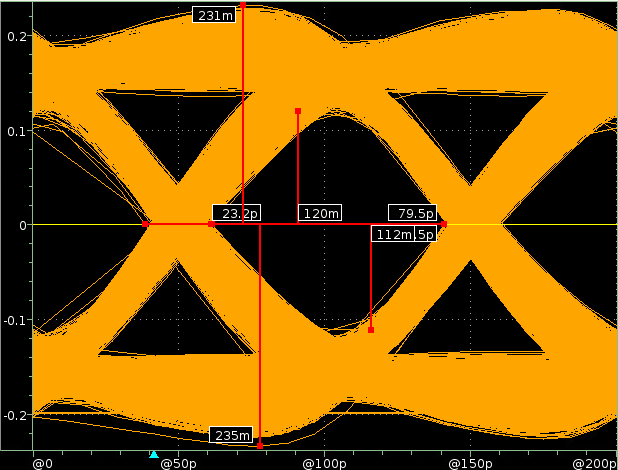
\includegraphics[width=\linewidth]{chapter4/pre_ext/eyes/with_channel/EQ3/EQ3_TT_Rmax.png}
		\caption{Res\_max}\label{fig:eye_EQ3_TT_Rmax}
	\end{subfigure}
	\caption{EQ3 eye diagrams for resistor corners at \ac{TT}}\label{fig:eye_EQ3_TT}
\end{figure}

\begin{table}[H]
 \centering
 \caption{EQ3 \ac{RX} eye diagram metrics across resistor corners at \ac{TT}}
 \label{tab:eq3_eye_res_TT}
 \begin{tabular}{ccc}
  \hline \hline
  \textbf{Corner} & \textbf{Height} & \textbf{Width} \\
  \hline 
  Res\_min & \SI{206}{\milli\volt} & \SI{78.9}{\pico\second} \\
  Res\_nom & \SI{231}{\milli\volt} & \SI{79.6}{\pico\second} \\
  Res\_max & \SI{232}{\milli\volt} & \SI{79.5}{\pico\second} \\
  \hline \hline
 \end{tabular}
\end{table}

The corresponding EQ3 resistor-corner eye diagrams at \ac{FF} are shown in Figure~\ref{fig:eye_EQ3_FF}.

\begin{figure}[H]
  \centering
	\begin{subfigure}{0.49\textwidth}
		\centering
		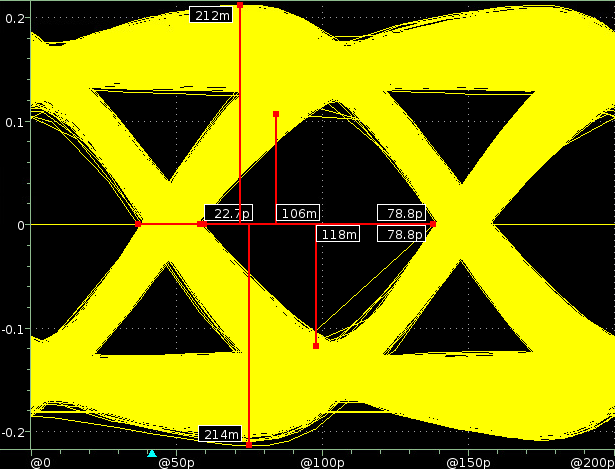
\includegraphics[width=\linewidth]{chapter4/pre_ext/eyes/with_channel/EQ3/EQ3_FF_Rmin.png}
		\caption{Res\_min}\label{fig:eye_EQ3_FF_Rmin}
	\end{subfigure}
	\begin{subfigure}{0.49\textwidth}
		\centering
		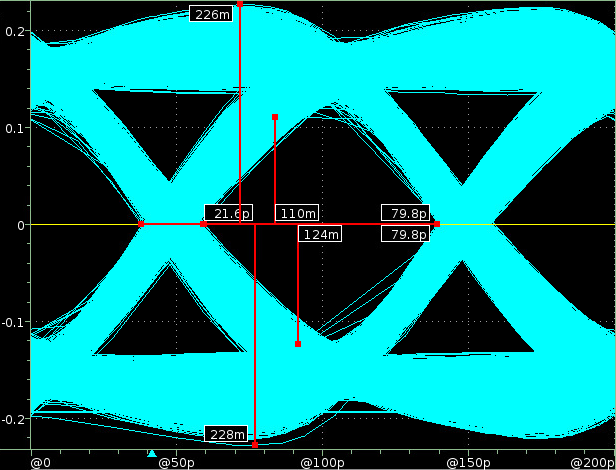
\includegraphics[width=\linewidth]{chapter4/pre_ext/eyes/with_channel/EQ3/EQ3_FF_Rnom.png}
		\caption{Res\_nom}\label{fig:eye_EQ3_FF_Rnom}
	\end{subfigure}
	\begin{subfigure}{0.49\textwidth}
		\centering
		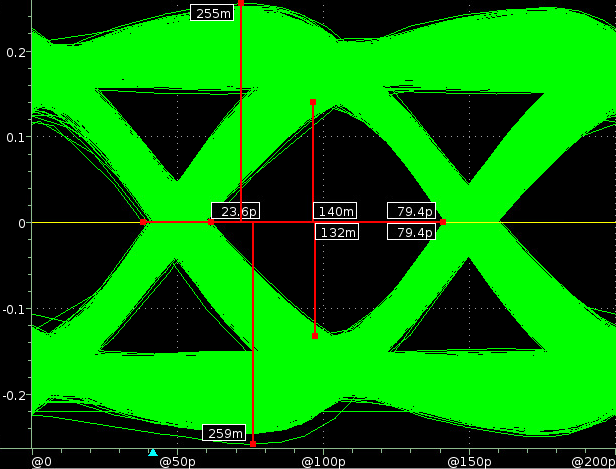
\includegraphics[width=\linewidth]{chapter4/pre_ext/eyes/with_channel/EQ3/EQ3_FF_Rmax.png}
		\caption{Res\_max}\label{fig:eye_EQ3_FF_Rmax}
	\end{subfigure}
	\caption{EQ3 eye diagrams for resistor corners at \ac{FF}}\label{fig:eye_EQ3_FF}
\end{figure}

\begin{table}[H]
 \centering
 \caption{EQ3 \ac{RX} eye diagram metrics across resistor corners at \ac{FF}}
 \label{tab:eq3_eye_res_FF}
 \begin{tabular}{ccc}
  \hline \hline
  \textbf{Corner} & \textbf{Height} & \textbf{Width} \\
  \hline 
  Res\_min & \SI{224}{\milli\volt} & \SI{78.8}{\pico\second} \\
  Res\_nom & \SI{234}{\milli\volt} & \SI{79.8}{\pico\second} \\
  Res\_max & \SI{272}{\milli\volt} & \SI{79.4}{\pico\second} \\
  \hline \hline
 \end{tabular}
\end{table}

The corresponding EQ3 resistor-corner eye diagrams at \ac{SS} are shown in Figure~\ref{fig:eye_EQ3_SS}.

\begin{figure}[H]
  \centering
	\begin{subfigure}{0.49\textwidth}
		\centering
		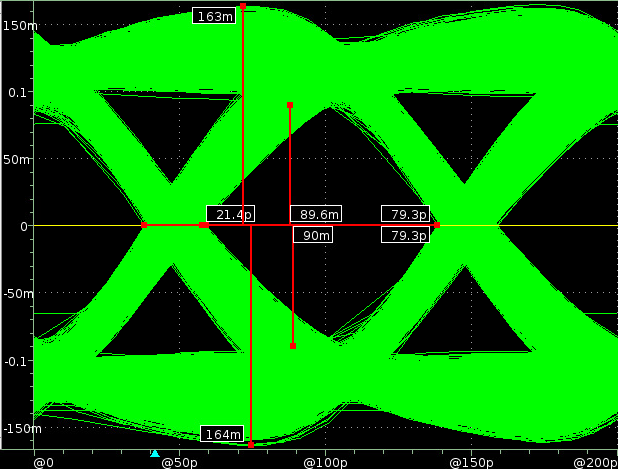
\includegraphics[width=\linewidth]{chapter4/pre_ext/eyes/with_channel/EQ3/EQ3_SS_Rmin.png}
		\caption{Res\_min}\label{fig:eye_EQ3_SS_Rmin}
	\end{subfigure}
	\begin{subfigure}{0.49\textwidth}
		\centering
		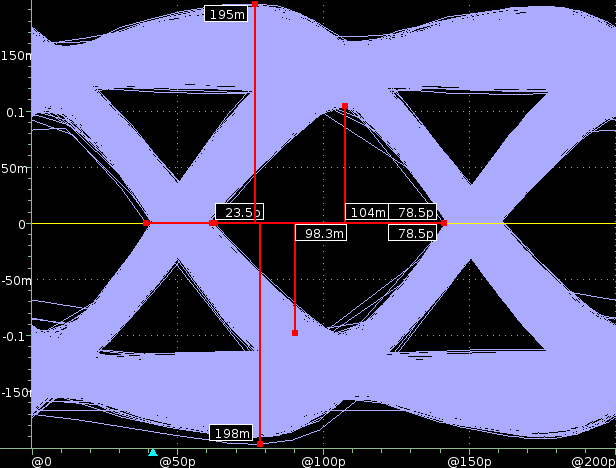
\includegraphics[width=\linewidth]{chapter4/pre_ext/eyes/with_channel/EQ3/EQ3_SS_Rnom.png}
		\caption{Res\_nom}\label{fig:eye_EQ3_SS_Rnom}
	\end{subfigure}
	\begin{subfigure}{0.49\textwidth}
		\centering
		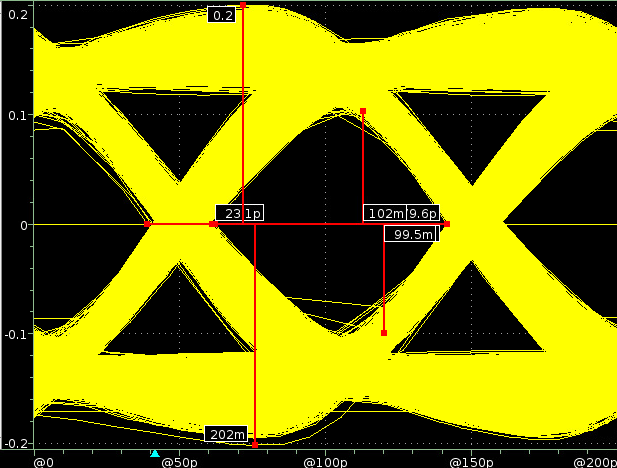
\includegraphics[width=\linewidth]{chapter4/pre_ext/eyes/with_channel/EQ3/EQ3_SS_Rmax.png}
		\caption{Res\_max}\label{fig:eye_EQ3_SS_Rmax}
	\end{subfigure}
	\caption{EQ3 eye diagrams for resistor corners at \ac{SS}}\label{fig:eye_EQ3_SS}
\end{figure}

\begin{table}[H]
 \centering
 \caption{EQ3 \ac{RX} eye diagram metrics across resistor corners at \ac{SS}}
 \label{tab:eq3_eye_res_SS}
 \begin{tabular}{ccc}
  \hline \hline
  \textbf{Corner} & \textbf{Height} & \textbf{Width} \\
  \hline
  Res\_min & \SI{179.6}{\milli\volt} & \SI{79.3}{\pico\second} \\
  Res\_nom & \SI{202.3}{\milli\volt} & \SI{78.5}{\pico\second} \\
  Res\_max & \SI{201.5}{\milli\volt} & \SI{79.6}{\pico\second} \\
  \hline \hline
 \end{tabular}
\end{table}

    %\subparagraph{Impact on impedance matching}
    %\subsubsection{Resistor Process Corners}
    %\paragraph{Analysis for Res Corners only}
        %\subparagraph{Eye diagram}
        %\subparagraph{Impact on impedance matching}
%\subsection{Full Process Variation}
      %\paragraph{Analysis for PVT and Res corners}
        %\subparagraph{Eye diagram}
        %\subparagraph{Impact on impedance matching}
\subsection{Power Consumption}

The power consumption of the transmitter driver was evaluated at the EQ3 equalization preset across all three \ac{PVT} corners considered, with the supply current and corner-dependent supply voltage used to compute the resulting static power dissipation, following the general relationship

\begin{equation}
  P = I_{DD} \cdot V_{DD}.
  \label{eq:pvi}
\end{equation}

As expected, the power consumption follows the combined trend of supply current and supply voltage across corners, reaching its maximum at the \ac{FF} corner, where both the current sunk by the driver and the supply voltage are at their highest, and its minimum at the \ac{SS} corner, where both quantities are at their lowest. The resulting power consumption values are summarized in Table~\ref{tab:power_consumption}.

\begin{table}[htbp]
 \centering
 \caption{Driver power consumption for EQ3}
 \label{tab:power_consumption}
 \begin{tabular}{cccc}
  \hline \hline
  \textbf{Corners} & \textbf{$\mathrm{I_{DD}}$} & \textbf{$\mathrm{V_{DD}}$} & \textbf{P}\\
  \hline
  \ac{TT}, Res\_nom & \SI{21.2}{\milli\ampere} & \SI{1.2}{\volt} & \SI{25.5}{\milli\watt} \\
  \ac{TT}, Res\_min & \SI{21.4}{\milli\ampere} & \SI{1.2}{\volt} & \SI{25.6}{\milli\watt} \\
  \ac{TT}, Res\_max & \SI{21.1}{\milli\ampere} & \SI{1.2}{\volt} & \SI{25.3}{\milli\watt} \\
  \ac{FF}, Res\_nom & \SI{21.8}{\milli\ampere} & \SI{1.26}{\volt} & \SI{27.4}{\milli\watt} \\
  \ac{FF}, Res\_min & \SI{21.9}{\milli\ampere} & \SI{1.26}{\volt} & \SI{27.6}{\milli\watt} \\
  \ac{FF}, Res\_max & \SI{21.7}{\milli\ampere} & \SI{1.26}{\volt} & \SI{27.3}{\milli\watt} \\
  \ac{SS}, Res\_nom & \SI{20.2}{\milli\ampere} & \SI{1.14}{\volt} & \SI{23}{\milli\watt} \\
  \ac{SS}, Res\_min & \SI{20.4}{\milli\ampere} & \SI{1.14}{\volt} & \SI{23.3}{\milli\watt} \\
  \ac{SS}, Res\_max & \SI{20}{\milli\ampere} & \SI{1.14}{\volt} & \SI{22.9}{\milli\watt} \\
  \hline \hline
 \end{tabular}
\end{table}

\section{Post Extraction Results}\label{sec:pext_results}
 
The complete driver, including all tap unit instances, the current-mirror biasing cell, and the termination network, occupies a total layout area of \SI{176}{\micro\meter} $\times$ \SI{82}{\micro\meter}. To close the guard ring around the full extent of the driver, additional dummy cells had to be inserted along the boundary of the layout, beyond those already present within the individual tap unit standard cells described in Section~\ref{sec:tap_unit_layout}, in order to maintain a continuous, uninterrupted guard ring around the complete macro. The resulting full driver layout is shown in Figure~\ref{fig:driver_layout_full}.

\begin{figure}[H]
  \centering
  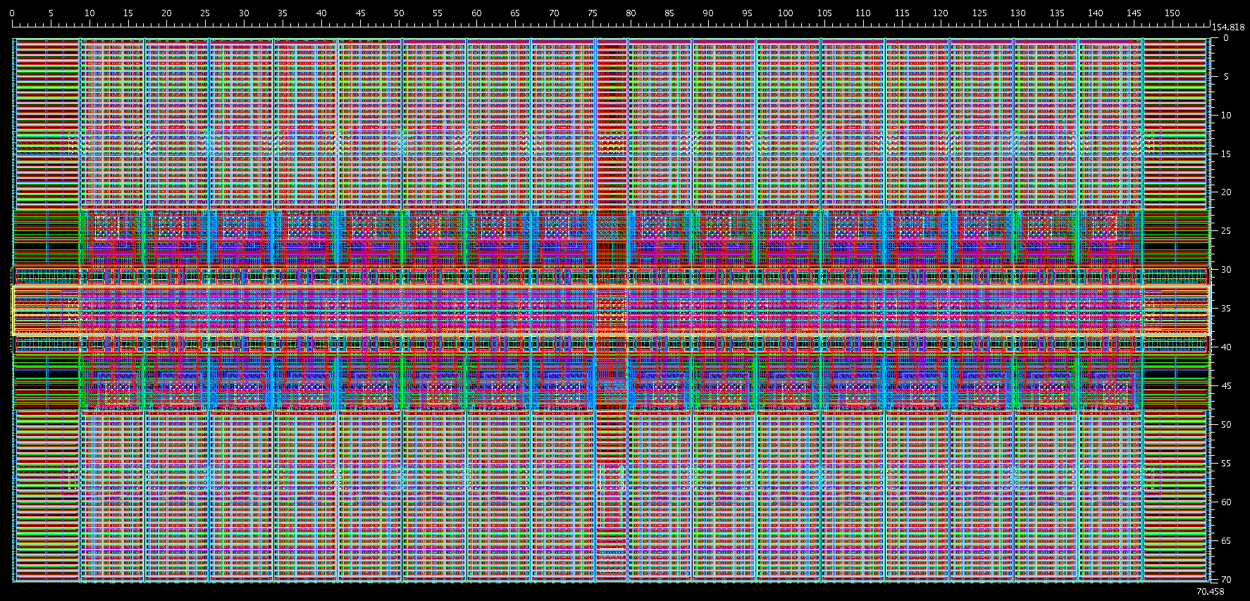
\includegraphics[width=0.9\textwidth]{chapter4/driver_layout_full.png}
  \caption{Complete driver layout }\label{fig:driver_layout_full}
\end{figure}

\subsection{Extracted Parasitic Capacitance and Coupling Analysis}
\label{sec:parasitic_capacitance_analysis}

%Following parasitic extraction of the completed layout, discussed in the context of the verification methodology in Section~\ref{sec:verification_methodology}, the extracted parasitic capacitances associated with the differential signal nets were analyzed to assess the degree of symmetry achieved between complementary net pairs, and to identify the dominant sources of parasitic coupling within the design.

The extracted total parasitic capacitances were found to be highly symmetrical across all differential net pairs in the design. The output nets, $TX_p$ and $TX_n$, exhibit a difference of only 0.98\% in total parasitic capacitance between the two branches. The pre-cursor tap nets, $PRE_p$ and $PRE_n$, exhibit a difference of 0.39\%, the post-cursor tap nets, $POST_p$ and $POST_n$, exhibit a difference of 1.29\%, and the main-cursor tap nets, $MAIN_p$ and $MAIN_n$, exhibit a difference of 0.41\%.

\begin{table}[htbp]
 \centering
 \caption{Differential nets parasitic capacitances}
 \label{tab:parasitic_capacitances}
 \begin{tabular}{cc}
  \hline \hline
  \textbf{Net} & \textbf{$\mathrm{C_{par}}$}\\
  \hline
  $\mathrm{TX_p}$ 		& 	\SI{340.17}{\femto\farad}		\\
  $\mathrm{TX_n}$ 		& 	\SI{336.87}{\femto\farad} 		\\
  $\mathrm{PRE_p}$ 		& 	\SI{17.9}{\femto\farad} 		\\
  $\mathrm{PRE_n}$ 		& 	\SI{17.97}{\femto\farad} 		\\
  $\mathrm{POST_p}$ 	& 	\SI{55.09}{\femto\farad} 		\\
  $\mathrm{POST_n}$ 	& 	\SI{55.8}{\femto\farad} 		\\
  $\mathrm{MAIN_p}$ 	& 	\SI{233.49}{\femto\farad}		\\
  $\mathrm{MAIN_n}$ 	& 	\SI{232.55}{\femto\farad} 		\\
  \hline \hline
 \end{tabular}
\end{table}

These results provide a quantitative confirmation of the effectiveness of the symmetry-first layout methodology adopted for the driver, in which the differential signal nets were prioritized above all other routing during the layout design process. The consistently low mismatch observed across all four differential net pairs, all below 1.3\%, demonstrates that this prioritization was effective in achieving a high degree of parasitic symmetry between the complmeentary branches of the differential signal path, which is essential for minimizing \ac{DCD} and timing skew, as discussed in Section~\ref{sec:jitter_detailed}.

\subsubsection{Dominant Net-to-Net Coupling}
\label{sec:net_coupling_analysis}

Beyond the overall symmetry of the total parasitic capacitance on each net, the extracted results were further analyzed to identify the dominant coupling capacitances between individual nets, summarized in Table~\ref{tab:net_coupling}.

\begin{table}[htbp]
  \centering
  \caption{Dominant coupled net and coupling capacitance for each differential net}
  \label{tab:net_coupling}
  \begin{tabular}{lccc}
    \hline \hline
    \textbf{Net} & \textbf{Highest Coupled Net} & \textbf{Coupling Cap} & \textbf{\% of net $\mathrm{C_{par}}$} \\
    \hline
    $\mathrm{TX_p}$  & $\mathrm{MAIN_n}$ & \SI{82.45}{\femto\farad} & 24.24\% \\
    $\mathrm{TX_n}$  & $\mathrm{MAIN_p}$ & \SI{80.25}{\femto\farad} & 23.82\% \\
    $\mathrm{PRE_p}$ & $\mathrm{TX_p}$  & \SI{6.78}{\femto\farad} & 37.91\% \\
    $\mathrm{PRE_n}$ & $\mathrm{TX_n}$  & \SI{6.75}{\femto\farad} & 37.58\% \\
    $\mathrm{POST_p}$ & $\mathrm{TX_p}$  & \SI{20.36}{\femto\farad} & 36.96\% \\
    $\mathrm{POST_n}$ & $\mathrm{TX_n}$  & \SI{20.27}{\femto\farad} & 36.33\% \\
    $\mathrm{MAIN_p}$ & $\mathrm{TX_n}$  & \SI{80.25}{\femto\farad} & 34.37\% \\
    $\mathrm{MAIN_n}$ & $\mathrm{TX_p}$  & \SI{82.45}{\femto\farad} & 35.45\% \\
    \hline \hline
  \end{tabular}
\end{table}

These results are a direct consequence of the metal layers used, and placement of the differential nets within the layout. The use of \ac{M5} for $TX_p$ and $TX_n$, and \ac{M4} for the tap input nets make them prone to coupling with each other when overlapped. Figure~\ref{fig:layout_IN_TX} shows a close-up view of the differential pair, highlighting the overlap between the differential output nets and the tap input nets.

\begin{figure}[H]
	\centering
	\begin{subfigure}[c]{0.3\linewidth}
		\centering
		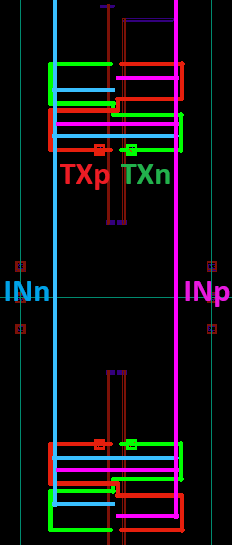
\includegraphics[width=\linewidth]{chapter4/post_ext/layout/PREn_BLU_PREp_PNK_TXn_GRN_TXp_RED_1.png}
		\caption{Pre-cursor tap input and output routing}\label{fig:layout_PRE_TX}
	\end{subfigure}
	\begin{subfigure}[c]{0.6\linewidth}
		\centering
		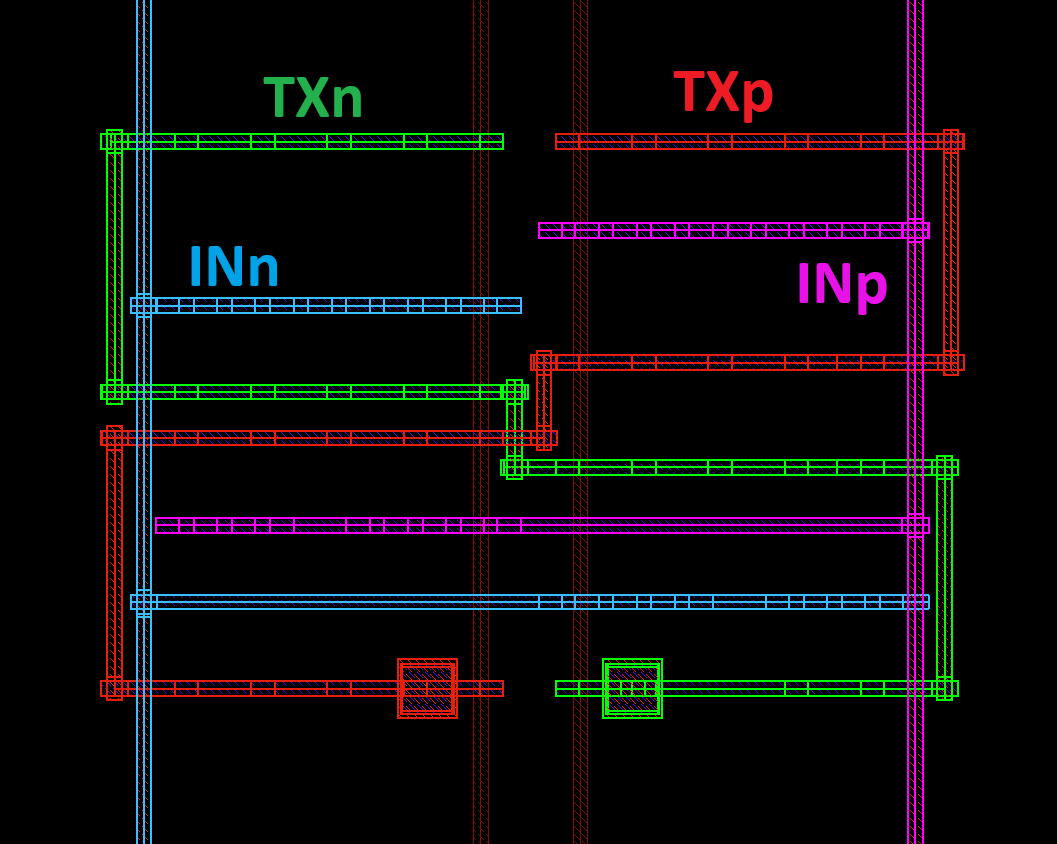
\includegraphics[width=0.7\linewidth]{chapter4/post_ext/layout/closeup_IN_TX.png}
		\caption{Post-cursor tap input and output routing}\label{fig:layout_POST_TX}
	\end{subfigure}
	\caption{Differential pair input and output routing}\label{fig:layout_IN_TX}
\end{figure}
	
At the center of the differential pair, an overlap between $TX_p$ and $TX_n$ is observed, due to the common-centroid matching chosen for these devices during floorplanning. It was known that these nets would have at least one point of overlap, and the routing of the tap unit was designed to minimize the overlapping of these input nets. The extracted parasitics show that, even though this overlap was minimized as much as possible, the existence of this overlap on every single tap unit cell adds up to a significant portion of the total parasitic capacitance on these nets, with $TX_p$ and $TX_n$ amounting to around 14\% of the total parasitic on each other, the second highest for both.

On the side edges, the tap input nets are placed, with seven overlapping points between input and output nets of the same polarity. %This explains the dominance of the coupling between the plus and minus nets for the pre and post taps, but this tendency is not observed for the main tap. 

\subsection{Post Extraction Performance}\label{sec:post_extraction_performance}


With no equalization applied, corresponding to the EQ0 preset, the driver achieves a post-extraction differential output voltage swing of $1.28\,\text{V}_{pp}$ at the \ac{FF} corner, $1.1\,\text{V}_{pp}$ at the \ac{TT} corner, and $0.908\,\text{V}_{pp}$ at the \ac{SS} corner. Figure~\ref{fig:vo_swing_PVT_EQ0_pext} shows the resulting differential output voltage swing across all three \ac{PVT} corners for the EQ0 preset.

\begin{figure}[h]
	\centering
	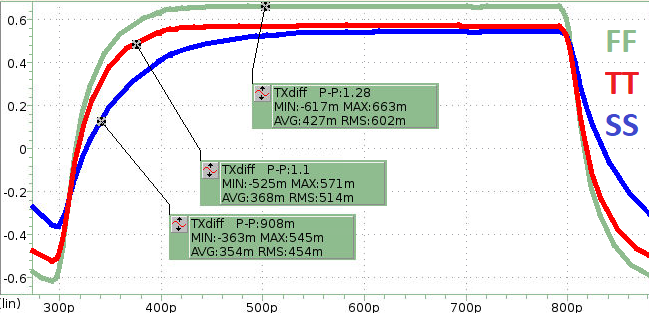
\includegraphics[width=0.8\linewidth]{chapter4/post_ext/Vo_swing/PVT_EQ0.png}
	\caption{Differential output voltage swing across \ac{PVT} corners for EQ0}\label{fig:vo_swing_PVT_EQ0_pext}
\end{figure}

The post-extraction \ac{PS} and \ac{DE} results for the four equalized presets (EQ1--EQ4), evaluated across all three \ac{PVT} corners, are summarized in Table~\ref{tab:PVT_eq_results_pext}. Table~\ref{tab:PVT_eq_results_pext_deviation} expresses the same results as the percentage deviation from the nominal target defined for each preset. For consistency with the target values used throughout this chapter, \ac{DE} is reported as a positive magnitude in the following tables.

\begin{table}[htbp]
	\centering
	\caption{Post-extraction equalization results across \ac{PVT} corners}
	\label{tab:PVT_eq_results_pext}
	\begin{tabular}{cccc}
	\hline \hline
	\textbf{Preset} & \textbf{Corner} & \textbf{PS} & \textbf{DE} \\
	\hline
	EQ1 & TT\_Rnom & 1.317 & 1.426 \\
	EQ1 & FF\_Rnom & 1.246 & 1.468 \\
	EQ1 & SS\_Rnom & 1.39 & 1.41 \\

	EQ2 & TT\_Rnom & 2.159 & 2.346 \\
	EQ2 & FF\_Rnom & 2.065 & 2.344 \\
	EQ2 & SS\_Rnom & 1.996 & 0.315 \\

	EQ3 & TT\_Rnom & 3.121 & 6.114 \\
	EQ3 & FF\_Rnom & 3.086 & 6.100 \\
	EQ3 & SS\_Rnom & 2.972 & 3.848 \\

	EQ4 & TT\_Rnom & 2.554 & 4.119 \\
	EQ4 & FF\_Rnom & 2.499 & 4.110 \\
	EQ4 & SS\_Rnom & 2.390 & 1.867 \\
	\hline \hline
	\end{tabular}
\end{table}

\begin{table}[htbp]
    \centering
    \caption{Post-extraction equalization results across \ac{PVT} corners,
    expressed as percentage deviation from target}
    \label{tab:PVT_eq_results_pext_deviation}
    \begin{tabular}{lcccccc}
        \hline \hline
        \textbf{Preset} &
        \multicolumn{2}{c}{\textbf{TT}} &
        \multicolumn{2}{c}{\textbf{FF}} &
        \multicolumn{2}{c}{\textbf{SS}} \\
        & \textbf{PS} & \textbf{DE}
        & \textbf{PS} & \textbf{DE}
        & \textbf{PS} & \textbf{DE} \\
        \hline
        EQ1 & +9.75\% & $-32.10\%$
            & +3.83\% & $-30.10\%$
            & +15.83\% & $-32.86\%$ \\

        EQ2 & $-1.85\%$ & $-24.32\%$
            & $-6.12\%$ & $-24.40\%$
            & $-9.29\%$ & $-89.85\%$ \\

        EQ3 & $-2.45\%$ & $-12.66\%$
            & $-3.56\%$ & $-12.86\%$
            & $-7.11\%$ & $-45.02\%$ \\

        EQ4 & +2.17\% & $-17.61\%$
            & $-0.05\%$ & $-17.80\%$
            & $-4.40\%$ & $-62.66\%$ \\
        \hline \hline
    \end{tabular}
\end{table}

The post-extraction results show that the layout does not affect all equalization metrics or \ac{PVT} corners equally. At the \ac{TT} and \ac{FF} corners, \ac{PS} remains comparatively close to its target for all four presets, whereas the \ac{DE} magnitude is systematically reduced. At the \ac{SS} corner, the degradation becomes substantially more pronounced for the stronger equalization presets. For EQ1, for example, the \ac{DE} magnitude decreases to 1.41~dB, corresponding to a 32.86\% reduction relative to its 2.1~dB target. More severe \ac{DE} reductions are observed for EQ2--EQ4 at \ac{SS}, reaching 89.85\% for EQ2, 45.02\% for EQ3, and 62.66\% for EQ4.

These results indicate that parasitic extraction modifies the effective relative weighting of the three \ac{FFE} tap currents. The effect is substantially more pronounced for \ac{DE} than for \ac{PS} and becomes particularly severe at the \ac{SS} corner. However, the sensitivity is not identical for all presets, indicating that the impact of the extracted parasitics depends on the particular current allocation between the pre-cursor, main-cursor, and post-cursor paths. The equalization results alone do not uniquely identify a single tap as the sole source of the error. Instead, they demonstrate that the nominal tap-current allocation derived at schematic level is not preserved uniformly across \ac{PVT} after extraction.

The resulting error also demonstrates the importance of the digitally segmented current-source architecture. Since the pre-cursor, main-cursor, and post-cursor currents can be adjusted independently, the tap-enable mapping can be retuned after extraction without modifying the underlying analog driver.

% - EQ1 shows the biggest deviation from target, especially for DE
% - In order to show how the tuning can improve performance for PVT variations, EQ1 was used as an example and the taps enable values were modified to reduce the equalization error
% - For FF and TT, two new mappings were found to reduce equalization error: 6 - 102 - 16 and 7 - 102 - 16 for both corners
% - 6-102-16 has the smallest deviation, but its PS is below the specification margin
% - 7-102-16 has a higher deviation, but both its PS and DE are within the specification margin
% - For SS, two different mappings were found to reduce equalization error: 4 - 90 - 20 and 4 - 82 - 20 
% - 4-90-20 has the smallest overall deviation, but its PS is below the specification margin
% - 4-82-20 has a higher deviation, but both its PS and DE are within the specification margin
% - the results for these changes are as follows:
%          Preset	Corner	PS	DE	Target PS	Target DE	Diff PS	Diff DE
%6 102 12	EQ1	FF	1.046	1.43	1.2	2.1	-12.83	-31.90
%6 102 12	EQ1	SS	1.004	0.144	1.2	2.1	-16.33	-93.14
%6 102 12	EQ1	TT	1.09	1.4	1.2	2.1	-9.17	-33.33
%6 102 16	EQ1	TT	1.148	2.124	1.2	2.1	-4.33	1.14
%7 102 16	EQ1	TT	1.382	2.153	1.2	2.1	15.17	2.52
%6 102 16	EQ1	FF	1.1	2.099	1.2	2.1	-8.33	-0.05
%7 102 16	EQ1	FF	1.32	2.124	1.2	2.1	10.00	1.14
%4 90 20	EQ1	SS	1.08156	2.15204	1.2	2.1	-9.87	2.48
%4 82 20	EQ1	SS	1.2027	2.5256	1.2	2.1	0.23	20.27
%figure tuning_pext_SS shows the difference that tuning has on the output signal. For the starting mapping, almost no preshoot is observed, leading to a very low DE. After tuning, the preshoot is increased, leading to a much better DE

EQ1 was selected as a representative case to evaluate the available post-layout tuning range. Among the evaluated presets, EQ1 exhibits the largest \ac{DE} deviation at the \ac{TT} and \ac{FF} corners, while still showing a significant reduction at \ac{SS}. It therefore provides a useful case for evaluating whether the segmented current-source architecture can recover the required equalization through digital reconfiguration and whether the required correction remains valid across \ac{PVT}.

For the tuning sweep, the starting EQ1, 7-102-12, configuration was first evaluated as a reference operating point. At \ac{TT}, this configuration produces \SI{1.317}{\decibel} of \ac{PS} and \SI{1.426}{\decibel} of \ac{DE}. Increasing the post-cursor contribution to obtain 6-102-16, named EQ1C, significantly reduces the equalization error, producing \SI{1.148}{\decibel} of \ac{PS} and \SI{2.124}{\decibel} of \ac{DE}. However, its \ac{PS} remains below the \SI{1.2}{\decibel} normative minimum. Increasing the pre-cursor enable count to obtain 7-102-16, named EQ1D, produces \SI{1.382}{\decibel} of \ac{PS} and \SI{2.153}{\decibel} of \ac{DE}. Although this configuration has a larger deviation from the nominal \ac{PS} target, both equalization metrics fall within their required ranges, and 7-102-16 is therefore selected for the \ac{TT} corner.

The same behaviour is observed at \ac{FF}. The 6-102-16 configuration gives \SI{1.1}{\decibel} of \ac{PS} and \SI{2.09}{\decibel} of \ac{DE}, providing very small \ac{DE} error but insufficient \ac{PS}. The 7-102-16 configuration instead produces \SI{1.32}{\decibel} of \ac{PS} and \SI{2.12}{\decibel} of \ac{DE}, placing both quantities within the normative range. Consequently, 7-102-16 is also selected at \ac{FF}

The \ac{SS} corner requires a substantially different current allocation. Starting from 7-102-12, the extracted driver produces \SI{1.39}{\decibel} of \ac{PS} and \SI{1.41}{\decibel} of \ac{DE}. The 4-90-20, named EQ1A, candidate recovers the \ac{DE} magnitude to \SI{2.152}{\decibel}, but its \SI{1.082}{\decibel} \ac{PS} remains below the normative minimum. Reducing the main-cursor enable count further results in the 4-82-20 configuration, named EQ1B, which produces \SI{1.203}{\decibel} of \ac{PS} and \SI{2.526}{\decibel} of \ac{DE}. Although its \ac{DE} exceeds the nominal EQ1 target, both quantities are within their normative specification ranges, making 4-82-20 the selected configuration for the \ac{SS} corner.
The effect of the evaluated EQ1 tap-enable mappings on the output waveform at each \ac{PVT} corner is illustrated in Figure~\ref{fig:tuning_pext_PVT}.

\begin{figure}[H]
  \centering
	\begin{subfigure}{0.4\textwidth}
		\centering
		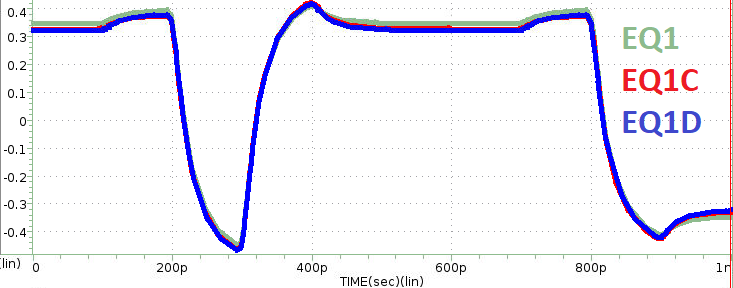
\includegraphics[width=\linewidth]{chapter4/post_ext/tuning/TT_EQ1_GRN_EQ1c_RED_EQ1d_BLU.png}
		\caption{\ac{TT}}\label{fig:tuning_pext_TT}
	\end{subfigure}
	\begin{subfigure}{0.4\textwidth}
		\centering
		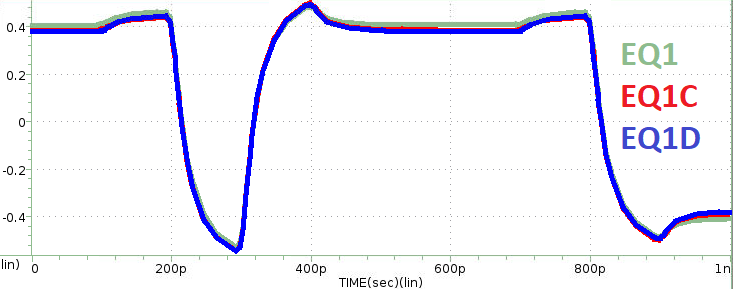
\includegraphics[width=\linewidth]{chapter4/post_ext/tuning/FF_EQ1_GRN_EQ1c_RED_EQ1d_BLU.png}
		\caption{\ac{FF}}\label{fig:tuning_pext_FF}
	\end{subfigure}
	\begin{subfigure}{0.4\textwidth}
		\centering
		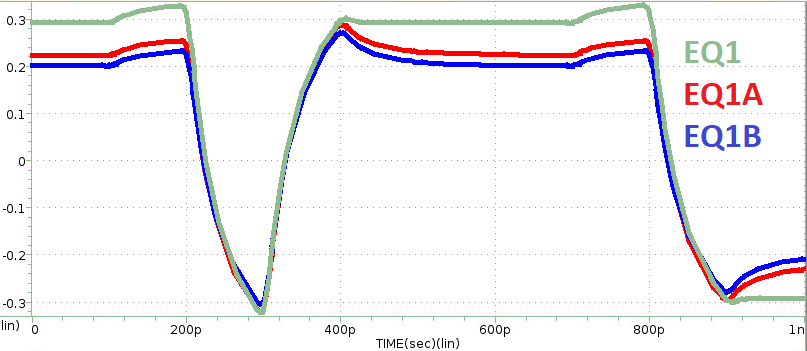
\includegraphics[width=\linewidth]{chapter4/post_ext/tuning/SS_EQ1_GRN_EQ1a_RED_EQ1b_BLU.png}
		\caption{\ac{SS}}\label{fig:tuning_pext_SS}
	\end{subfigure}
	\caption{Starting and tuned differential output for \ac{PVT} corners}\label{fig:tuning_pext_PVT}
\end{figure}


\begin{table}[htbp]
    \centering
    \caption{Post-extraction EQ1 target deviation before and after tap reconfiguration}
    \label{tab:eq1_tuning_comparison}
    \begin{tabular}{lcccccc}
        \hline \hline
		\textbf{Corner} & \textbf{Mapping} & \textbf{PS [dB]} & \textbf{DE [dB]} & \textbf{$\Delta$PS} & \textbf{$\Delta$DE} & \textbf{Result} \\
		\hline

	TT & EQ1 & 1.317 & 1.426 & $9.75\%$ & $-32.10\%$ & Reference \\
	TT & EQ1C & 1.148 & 2.124 & $-4.33\%$ & $+1.14\%$ &
	PS below minimum \\
	TT & \textbf{EQ1D} & \textbf{1.382} & \textbf{2.153} &
	\textbf{$+15.17\%$} & \textbf{$+2.52\%$} & \textbf{Selected} \\
	\hline

	FF & EQ1 & 1.246 & 1.468 & $+3.83\%$ & $-30.10\%$ & Reference \\
	FF & EQ1C & 1.100 & 2.099 & $-8.33\%$ & $-0.05\%$ &
	PS below minimum \\
	FF & \textbf{EQ1D} & \textbf{1.320} & \textbf{2.124} &
	\textbf{$+10.00\%$} & \textbf{$+1.14\%$} & \textbf{Selected} \\
	\hline

	SS & EQ1 & 1.39 & 1.41 & $+15.83\%$ & $-32.86\%$ & Reference \\
	SS & EQ1A & 1.082 & 2.152 & $-9.87\%$ & $+2.48\%$ &
	PS below minimum \\
	SS & \textbf{EQ1B} & \textbf{1.203} & \textbf{2.526} &
	\textbf{$+0.23\%$} & \textbf{$+20.27\%$} & \textbf{Selected} \\

	\hline \hline
	\end{tabular}
\end{table}

The tuning results show that minimizing the numerical deviation from the nominal EQ1 target is not by itself sufficient for selecting the final mapping. At both \ac{TT} and \ac{FF}, the 6-102-16 mapping gives the smallest overall target error, but its \ac{PS} remains below the normative minimum. The 7-102-16 mapping is therefore preferred because it places both \ac{PS} and \ac{DE} inside the allowed ranges. The same trade-off occurs at \ac{SS}, where 4-90-20 gives a smaller target error but insufficient \ac{PS}, whereas 4-82-20 provides a specification-compatible operating point.

Most importantly, the final mapping is not identical across \ac{PVT}: \ac{TT} and \ac{FF} are both corrected using 7-102-16, while \ac{SS} requires the substantially different 4-82-20 mapping. The segmented current-source architecture therefore provides sufficient tuning range to recover the required equalization after extraction, but the results also demonstrate that a single fixed EQ1 enable mapping is not robust across the full evaluated \ac{PVT} range. A practical implementation would consequently benefit from a calibration procedure or from pre-characterized corner-dependent configuration codes.

The post-extraction differential output-impedance sweeps across termination-bank settings and process corners are plotted in Figure~\ref{fig:zout_pext_PVT}.

\begin{figure}[H]
  \centering
	\begin{subfigure}{0.4\textwidth}
		\centering
		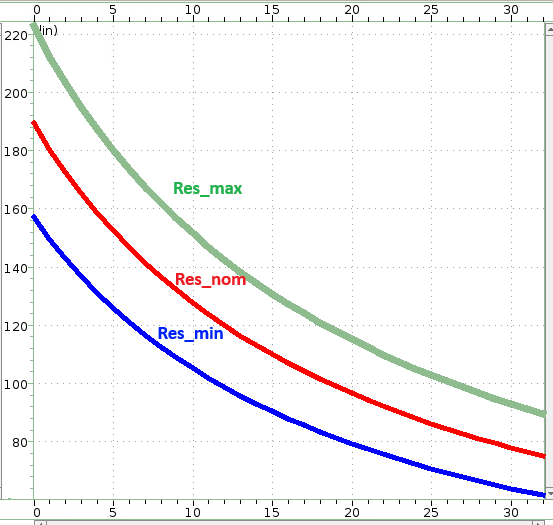
\includegraphics[width=\linewidth]{chapter4/post_ext/Zout/TT.png}
		\caption{\ac{TT}}\label{fig:zout_pext_TT_PVT}
	\end{subfigure}
	\begin{subfigure}{0.4\textwidth}
		\centering
		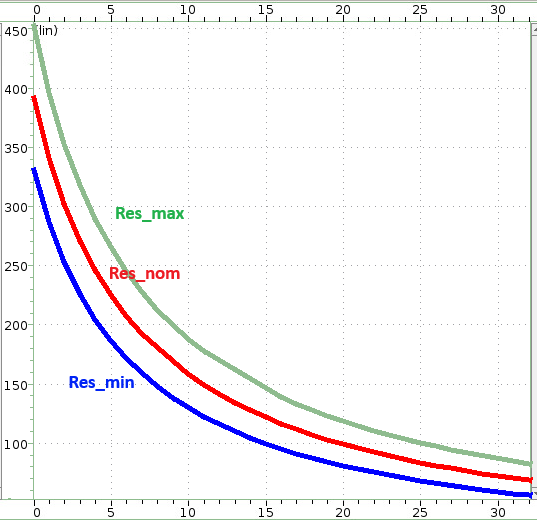
\includegraphics[width=\linewidth]{chapter4/post_ext/Zout/FF.png}
		\caption{\ac{FF}}\label{fig:zout_pext_FF_PVT}
	\end{subfigure}
	\begin{subfigure}{0.4\textwidth}
		\centering
		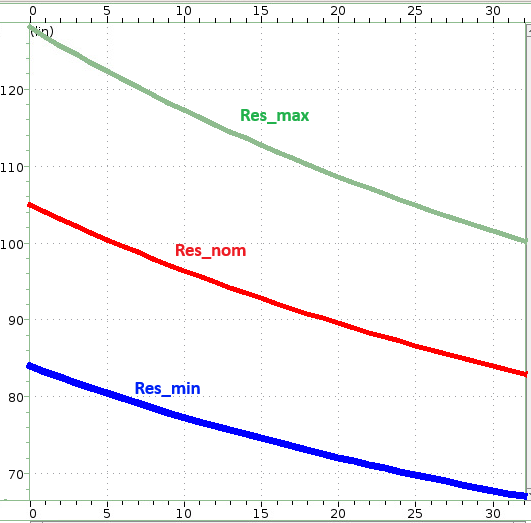
\includegraphics[width=\linewidth]{chapter4/post_ext/Zout/SS.png}
		\caption{\ac{SS}}\label{fig:zout_pext_SS_PVT}
	\end{subfigure}
	\caption{Post extraction differential output impedance across corners and bank configurations}\label{fig:zout_pext_PVT}
\end{figure}

\begin{table}[htbp]
 \centering
 \caption{Post extraction $\mathrm{Z_{out, diff}}$ across \ac{PVT} and resistor corners}
 \label{tab:zout_PVT_pext}
 \begin{tabular}{cccccc}
  \hline \hline
  \textbf{PVT} & \textbf{Res} & \textbf{\#$\mathrm{en_{max}}$} & \textbf{\#$\mathrm{en_{nom}}$} & \textbf{\#$\mathrm{en_{min}}$}\\
  \hline
  TT & Res\_min & 6 & 12 & 24\\
  TT & Res\_nom & 13 & 19 & 32\\
  TT & Res\_max & 19 & 27 & NA\\
  SS & Res\_min & NA & NA & 22\\ % SS Rmin cai muito rápido
  SS & Res\_nom & NA & 6 & NA\\
  SS & Res\_max & 9 & 32 & NA\\
  FF & Res\_min & 12 & 15 & NA\\
  FF & Res\_nom & 16 & 20 & NA\\
  FF & Res\_max & 20 & 26 & NA\\
  \hline \hline
 \end{tabular}
\end{table}

The post-extraction termination results show that a compliant differential output impedance can be obtained for every evaluated combination of \ac{PVT} and resistor corner by selecting an appropriate termination-bank enable count.
However, the complete \SIrange{72}{120}{\ohm} tuning interval is not reproduced at every combined corner, as indicated by the unavailable entries in Table~\ref{tab:zout_PVT_pext}. The extracted implementation should therefore be interpreted as providing at least one specification-compatible termination setting at each evaluated corner, rather than providing the complete normative impedance range under every condition.

The required enable count also changes substantially with process and resistor variation. For example, at \ac{TT} and Res\_nom, the nominal impedance point moves from 15 enabled termination elements before extraction to 19 after extraction. This shift further demonstrates that the programmable termination network is required not only to accommodate process variation, but also to compensate for the resistance and interconnect parasitics introduced by the physical implementation.

The post-extraction rise and fall waveforms for the three \ac{PVT} corners are shown in Figure~\ref{fig:rise_fall_PVT_pext}.

\begin{figure}[H]
  \centering
	\begin{subfigure}{0.32\textwidth}
		\centering
		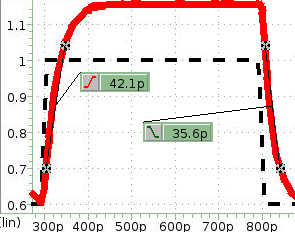
\includegraphics[width=\linewidth]{chapter4/post_ext/rise_fall_times/TT.png}
		\caption{\ac{TT}}\label{fig:rise_fall_TT_pext}
	\end{subfigure}
	\begin{subfigure}{0.32\textwidth}
		\centering
		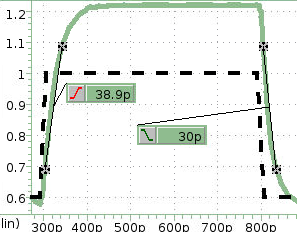
\includegraphics[width=\linewidth]{chapter4/post_ext/rise_fall_times/FF.png}
		\caption{\ac{FF}}\label{fig:rise_fall_FF_pext}
	\end{subfigure}
	\begin{subfigure}{0.32\textwidth}
		\centering
		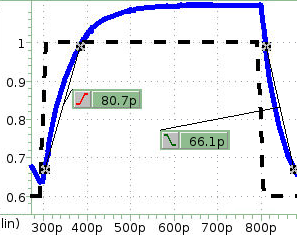
\includegraphics[width=\linewidth]{chapter4/post_ext/rise_fall_times/SS.png}
		\caption{\ac{SS}}\label{fig:rise_fall_SS_pext}
	\end{subfigure}
	\caption{Rise and fall times across \ac{PVT} corners}\label{fig:rise_fall_PVT_pext}
\end{figure}

\begin{table}[htbp]
 \centering
 \caption{Post extraction rise and fall times across \ac{PVT} corners}
 \label{tab:rise_fall_PVT_pext}
 \begin{tabular}{ccc}
  \hline \hline
  \textbf{Corner} & \textbf{Rise} & \textbf{Fall} \\
  \hline
  TT & \SI{42.1}{\pico\second} & \SI{35.6}{\pico\second} \\
  FF & \SI{38.9}{\pico\second} & \SI{30}{\pico\second} \\
  SS & \SI{80.7}{\pico\second} & \SI{66.1}{\pico\second} \\
  \hline \hline
 \end{tabular}
\end{table}

The post-extraction rise and fall times increase at all three PVT corners, consistent with the additional capacitive loading introduced by the extracted interconnect and device parasitics discussed in Section~4.3.1. At \ac{TT}, the rise time increases from 27.3~ps before extraction to 42.1~ps after extraction, while the fall time increases from 22.8~ps to 35.6~ps. These correspond to increases of approximately 54.2\% and 56.1\%, respectively.

The extracted \ac{SS} corner exhibits the slowest transitions, with a rise time of 80.7~ps and a fall time of 66.1~ps. Thus, although all measured transition times remain below the nominal 100~ps \ac{UI}, the reduction in transition-speed margin after extraction is significant, particularly at \ac{SS}. The persistent difference between rise and fall times is consistent with the asymmetric loading of the active \ac{PDN} and passive \ac{PUN} paths discussed previously.

At \ac{TT}, the post-extraction eye diagrams demonstrate a clear dependence of the received signal quality on the applied transmitter equalization. Table~\ref{tab:rx_eye_pvt_pext} summarizes the corresponding \ac{TX} and \ac{RX} eye metrics.


The post-extraction EQ0 \ac{TX} and \ac{RX} eye diagrams are presented in Figure~\ref{fig:eye_TT_EQ0_pext}.

\begin{figure}[H]
  \centering
	\begin{subfigure}{0.8\textwidth}
		\centering
		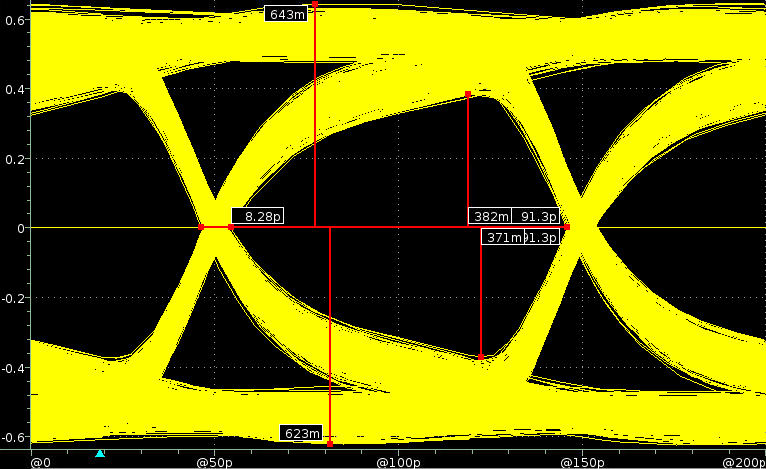
\includegraphics[width=\linewidth]{chapter4/post_ext/eyes/with_channel/EQ0_TT_TX.png}
		\caption{\ac{TX}}\label{fig:eye_TT_EQ0_TX_pext}
	\end{subfigure}
	\centering
	\begin{subfigure}{0.8\textwidth}
		\centering
		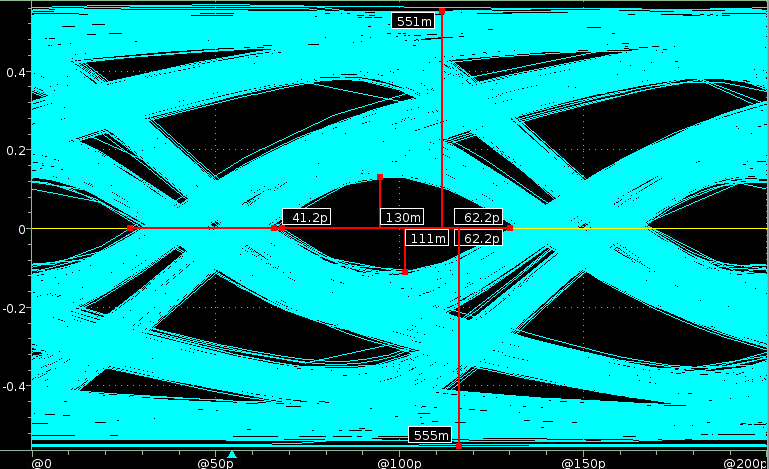
\includegraphics[width=\linewidth]{chapter4/post_ext/eyes/with_channel/EQ0_TT_RX.png}
		\caption{\ac{RX}}\label{fig:eye_TT_EQ0_RX_pext}
	\end{subfigure}
	\caption{Post extraction eye diagrams for EQ0 at corner \ac{TT}}\label{fig:eye_TT_EQ0_pext}
\end{figure}

For EQ0, the \ac{RX} eye has a height of \SI{241}{\milli\volt} and a width of \SI{62.2}{\pico\second}. Although a vertical opening remains after transmission through the reference channel, EQ0 provides the smallest horizontal opening of all evaluated post-extraction configurations.

The corresponding post-extraction EQ1 eye diagrams are shown in Figure~\ref{fig:eye_TT_EQ1_pext}.

\begin{figure}[H]
  \centering
	\begin{subfigure}{0.8\textwidth}
		\centering
		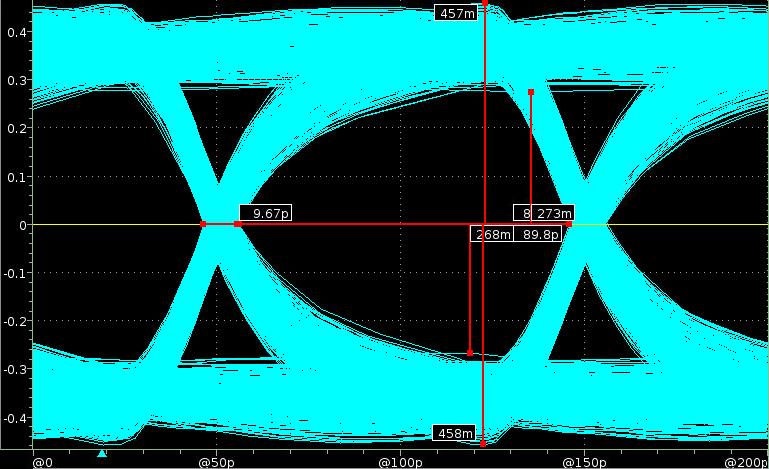
\includegraphics[width=\linewidth]{chapter4/post_ext/eyes/with_channel/EQ1_TT_TX.png}
		\caption{\ac{TX}}\label{fig:eye_TT_EQ1_TX_pext}
	\end{subfigure}
	\centering
	\begin{subfigure}{0.8\textwidth}
		\centering
		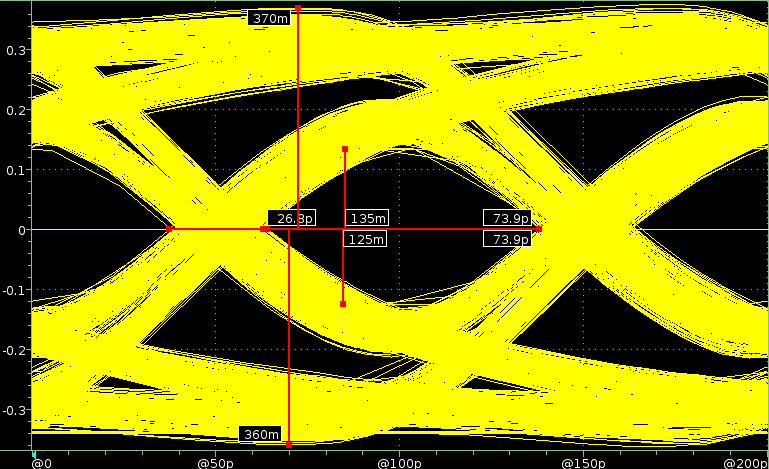
\includegraphics[width=\linewidth]{chapter4/post_ext/eyes/with_channel/EQ1_TT_RX.png}
		\caption{\ac{RX}}\label{fig:eye_TT_EQ1_RX_pext}
	\end{subfigure}
	\caption{Post extraction eye diagrams for EQ1 at corner \ac{TT}}\label{fig:eye_TT_EQ1_pext}
\end{figure}

Applying equalization progressively increases the \ac{RX} eye opening. EQ1 produces an \ac{RX} eye height of \SI{260}{\milli\volt} and a width of \SI{73.9}{\pico\second}, while EQ2 increases these values to \SI{296}{\milli\volt} and \SI{76}{\pico\second}, respectively.

The corresponding post-extraction EQ2 eye diagrams are shown in Figure~\ref{fig:eye_TT_EQ2_pext}.

\begin{figure}[H]
  \centering
	\begin{subfigure}{0.8\textwidth}
		\centering
		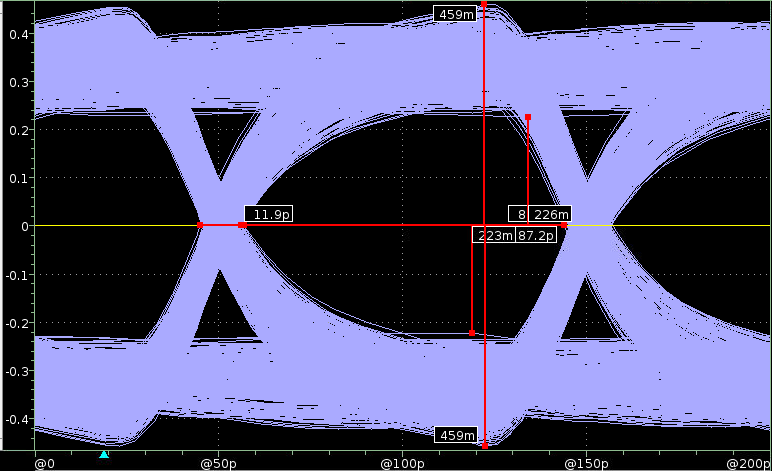
\includegraphics[width=\linewidth]{chapter4/post_ext/eyes/with_channel/EQ2_TT_TX.png}
		\caption{\ac{TX}}\label{fig:eye_TT_EQ2_TX_pext}
	\end{subfigure}
	\centering
	\begin{subfigure}{0.8\textwidth}
		\centering
		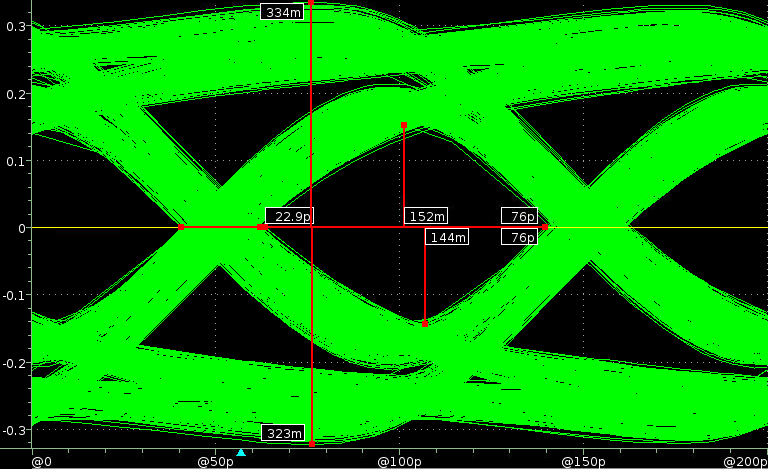
\includegraphics[width=\linewidth]{chapter4/post_ext/eyes/with_channel/EQ2_TT_RX.png}
		\caption{\ac{RX}}\label{fig:eye_TT_EQ2_RX_pext}
	\end{subfigure}
	\caption{Post extraction eye diagrams for EQ2 at corner \ac{TT}}\label{fig:eye_TT_EQ2_pext}
\end{figure}

The corresponding post-extraction EQ3 eye diagrams are shown in Figure~\ref{fig:eye_TT_EQ3_pext}.

\begin{figure}[H]
  \centering
	\begin{subfigure}{0.8\textwidth}
		\centering
		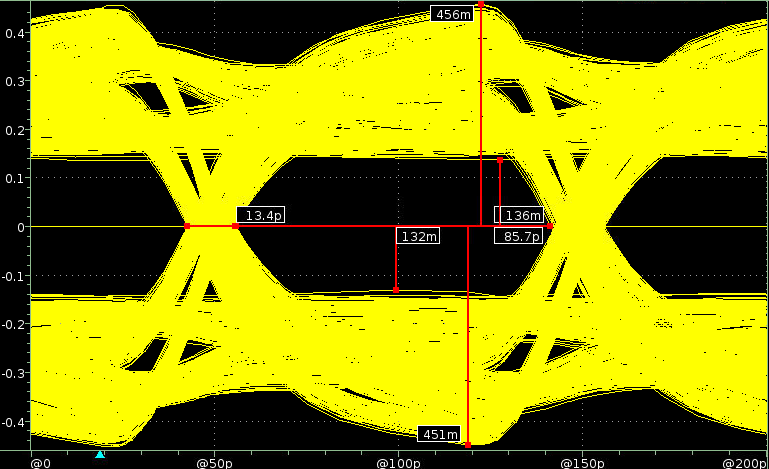
\includegraphics[width=\linewidth]{chapter4/post_ext/eyes/with_channel/EQ3_TT_TX.png}
		\caption{\ac{TX}}\label{fig:eye_TT_EQ3_TX_pext}
	\end{subfigure}
	\centering
	\begin{subfigure}{0.8\textwidth}
		\centering
		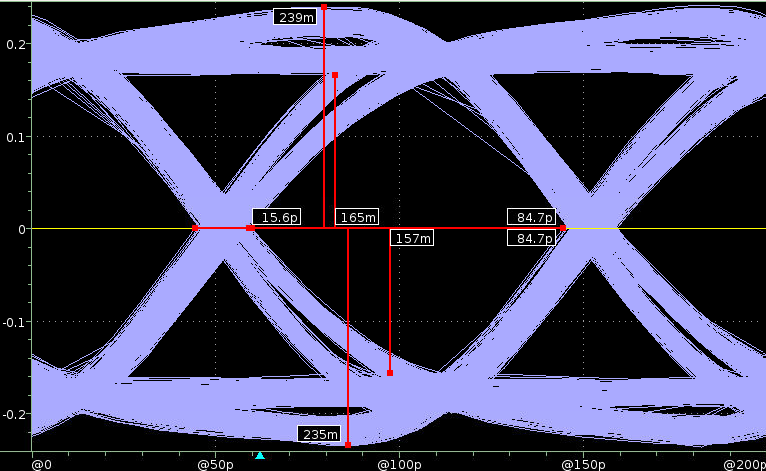
\includegraphics[width=\linewidth]{chapter4/post_ext/eyes/with_channel/EQ3_TT_RX.png}
		\caption{\ac{RX}}\label{fig:eye_TT_EQ3_RX_pext}
	\end{subfigure}
	\caption{Post extraction eye diagrams for EQ3 at corner \ac{TT}}\label{fig:eye_TT_EQ3_pext}
\end{figure}

The strongest eye openings are obtained with EQ3 and EQ4. EQ3 provides an \ac{RX} eye height of \SI{322}{\milli\volt} and an eye width of \SI{84.7}{\pico\second}, whereas EQ4 provides an eye height of \SI{323}{\milli\volt} and a width of \SI{84.3}{\pico\second}. The two configurations therefore provide essentially equivalent post-extraction performance: EQ4 gives the largest vertical opening by only \SI{1}{\milli\volt}, while EQ3 provides the largest horizontal opening by \SI{0.4}{\pico\second}.

The corresponding post-extraction EQ4 eye diagrams are shown in Figure~\ref{fig:eye_TT_EQ4_pext}.

\begin{figure}[H]
  \centering
	\begin{subfigure}{0.8\textwidth}
		\centering
		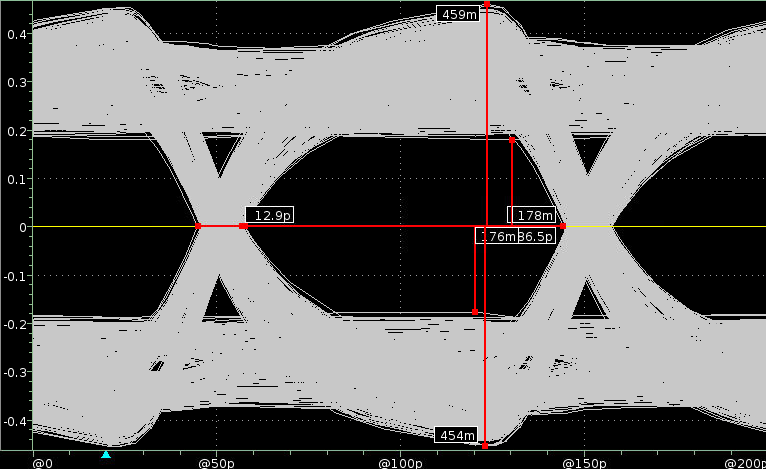
\includegraphics[width=\linewidth]{chapter4/post_ext/eyes/with_channel/EQ4_TT_TX.png}
		\caption{\ac{TX}}\label{fig:eye_TT_EQ4_TX_pext}
	\end{subfigure}
	\centering
	\begin{subfigure}{0.8\textwidth}
		\centering
		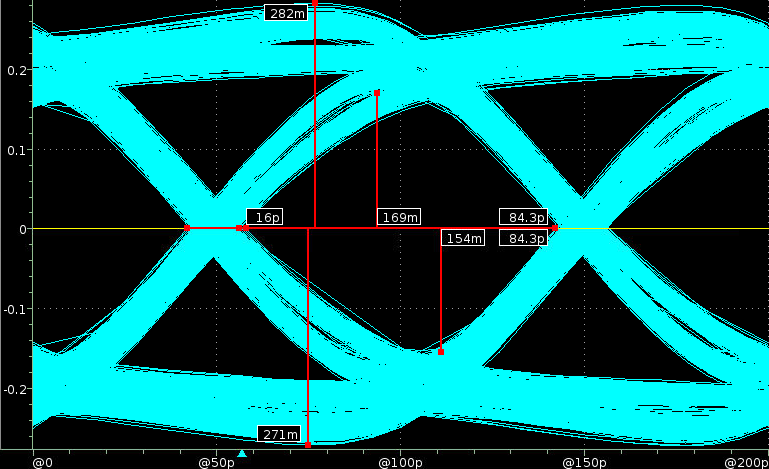
\includegraphics[width=\linewidth]{chapter4/post_ext/eyes/with_channel/EQ4_TT_RX.png}
		\caption{\ac{RX}}\label{fig:eye_TT_EQ4_RX_pext}
	\end{subfigure}
	\caption{Post extraction eye diagrams for EQ4 at corner \ac{TT}}\label{fig:eye_TT_EQ4_pext}
\end{figure}

EQ3 and EQ4 provide nearly identical post-extraction performance. EQ4 gives the marginally larger vertical eye opening (\SI{323}{\milli\volt} versus \SI{322}{\milli\volt}), whereas EQ3 provides both the marginally larger eye width (\SI{84.7}{\pico\second} versus \SI{84.3}{\pico\second}) and the slightly smaller crossover width (\SI{15.6}{\pico\second} versus \SI{16.0}{\pico\second}). Considering these metrics together, EQ3 is retained as the representative configuration for the detailed post-extraction corner analysis.

\begin{table}[htbp]
 \centering
 \caption{Post extraction eye metrics at \ac{TT} for different equalization presets}
 \label{tab:rx_eye_pvt_pext}
 \begin{tabular}{ccccc}
  \hline \hline
   \textbf{EQ} 	  & \textbf{TX} 	   & \textbf{TX}    & \textbf{RX} 	& \textbf{RX} \\
   \textbf{Preset} & \textbf{Height} & \textbf{Width} & \textbf{Height} & \textbf{Width}\\
  \hline
  EQ0 & \SI{699}{\milli\volt} 	& \SI{91.3}{\pico\second} 		& \SI{241}{\milli\volt} & \SI{62.2}{\pico\second}\\
  EQ1 & \SI{541}{\milli\volt} 	& \SI{89.8}{\pico\second} 		& \SI{260}{\milli\volt} & \SI{73.9}{\pico\second}\\
  EQ2 & \SI{449}{\milli\volt} 	& \SI{87.2}{\pico\second} 		& \SI{296}{\milli\volt} & \SI{76}{\pico\second}\\
  EQ3 & \SI{268}{\milli\volt} 	& \SI{85.7}{\pico\second} 		& \SI{322}{\milli\volt} & \SI{84.7}{\pico\second}\\
  EQ4 & \SI{354}{\milli\volt} 	& \SI{86.5}{\pico\second} 		& \SI{323}{\milli\volt} & \SI{84.3}{\pico\second}\\
  \hline \hline
 \end{tabular}
\end{table}

%\begin{figure}
  %  \centering
  %  \includegraphics[width=0.8\textwidth]{layout/DIFF_PAIR_FP_DIMS.png}
  %  \caption{\ac{RVT} devices floorplan boundary dimensions}\label{fig:RVT_fp_dims}
%\end{figure}

%\subsection{Extracted Parasitics}
%- extracted parasitics for the differential pair and the current source devices are shown in Table~\ref{tab:extracted_parasitics}
%\subsection{Pre and Post Extraction Comparison}
%\subsection{USB 3.2 Gen 2 Compliance}
%\subsection{Comparison with Existing Work}

Across the resistor-corner sweeps, the EQ3 \ac{RX} eye width remains relatively stable compared with the variation in eye height. At \ac{TT}, the measured eye width varies only from \SI{84.9}{\pico\second} to \SI{85.1}{\pico\second}, while the eye height varies from \SI{302}{\milli\volt} to \SI{334}{\milli\volt}. At \ac{FF}, the width remains between \SI{86.4}{\pico\second} and \SI{86.9}{\pico\second}, while the height ranges from \SI{359}{\milli\volt} to \SI{396}{\milli\volt}. At \ac{SS}, the width remains between \SI{83.1}{\pico\second} and \SI{84.9}{\pico\second}, whereas the height ranges from \SI{202.3}{\milli\volt} to \SI{221}{\milli\volt}.

The post-extraction EQ3 received eye diagrams at \ac{TT} for the three resistor corners are presented in Figure~\ref{fig:eye_EQ3_TT_pext}.

\begin{figure}[H]
\centering
\begin{subfigure}{0.4\textwidth}
	\centering
	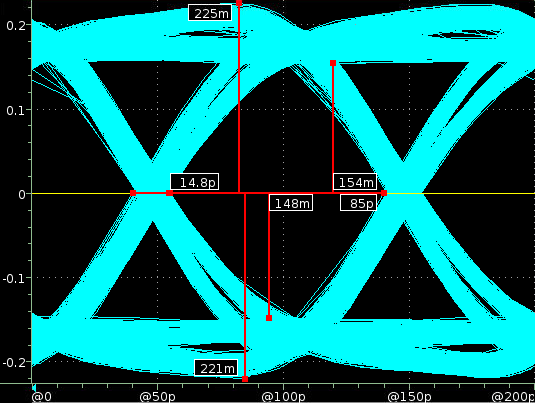
\includegraphics[width=\linewidth]{chapter4/post_ext/eyes/EQ3/EQ3_TT_Rmin.png}
	\caption{Res\_min}
\end{subfigure}
\begin{subfigure}{0.4\textwidth}
	\centering
	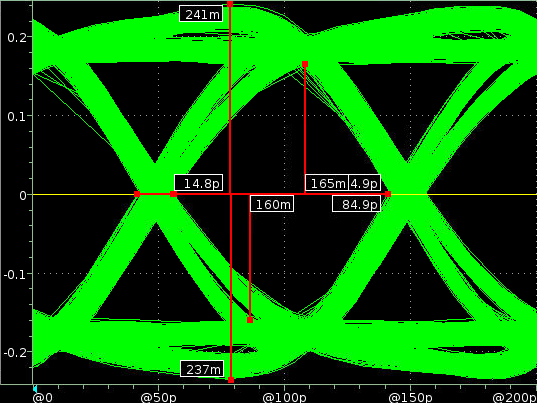
\includegraphics[width=\linewidth]{chapter4/post_ext/eyes/EQ3/EQ3_TT_Rnom.png}
	\caption{Res\_nom}
\end{subfigure}
\begin{subfigure}{0.4\textwidth}
	\centering
	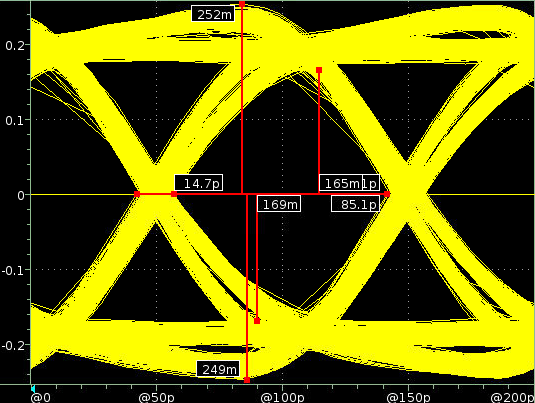
\includegraphics[width=\linewidth]{chapter4/post_ext/eyes/EQ3/EQ3_TT_Rmax.png}
	\caption{Res\_max}
\end{subfigure}
\caption{Post extraction EQ3 eye diagrams for resistor corners at \ac{TT}}\label{fig:eye_EQ3_TT_pext}
\end{figure}

\begin{table}[H]
 \centering
 \caption{Post extraction EQ3 \ac{RX} eye diagram metrics across resistor corners at \ac{TT}}
 \label{tab:eq3_eye_TT_pext}
 \begin{tabular}{ccc}
  \hline \hline
  \textbf{Corner} & \textbf{Height} & \textbf{Width} \\
  \hline
  Res\_min & \SI{302}{\milli\volt} & \SI{85}{\pico\second} \\
  Res\_nom & \SI{325}{\milli\volt} & \SI{84.9}{\pico\second} \\
  Res\_max & \SI{334}{\milli\volt} & \SI{85.1}{\pico\second} \\
  \hline \hline
 \end{tabular}
\end{table}

The corresponding post-extraction EQ3 eye diagrams at \ac{FF} are shown in Figure~\ref{fig:eye_EQ3_FF_pext}.

\begin{figure}[H]
\centering
\begin{subfigure}{0.4\textwidth}
	\centering
	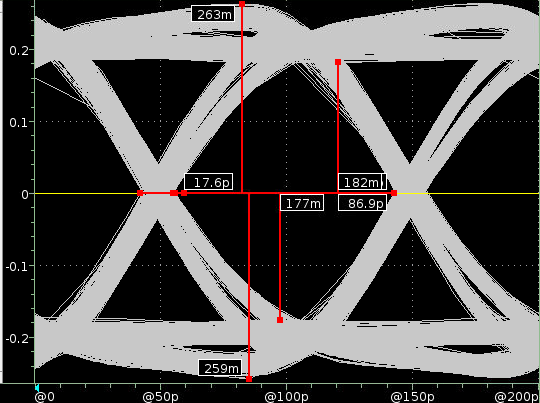
\includegraphics[width=\linewidth]{chapter4/post_ext/eyes/EQ3/EQ3_FF_Rmin.png}
	\caption{Res\_min}
\end{subfigure}
\begin{subfigure}{0.4\textwidth}
	\centering
	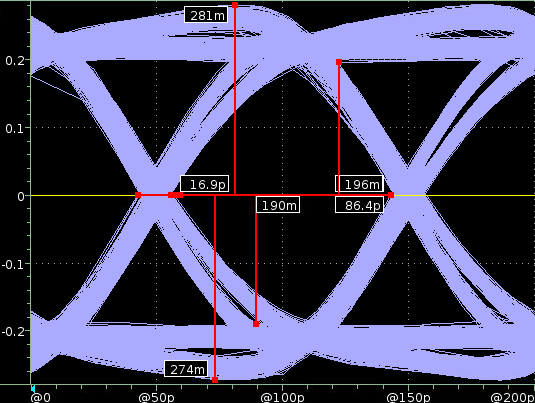
\includegraphics[width=\linewidth]{chapter4/post_ext/eyes/EQ3/EQ3_FF_Rnom.png}
	\caption{Res\_nom}
\end{subfigure}
\begin{subfigure}{0.4\textwidth}
	\centering
	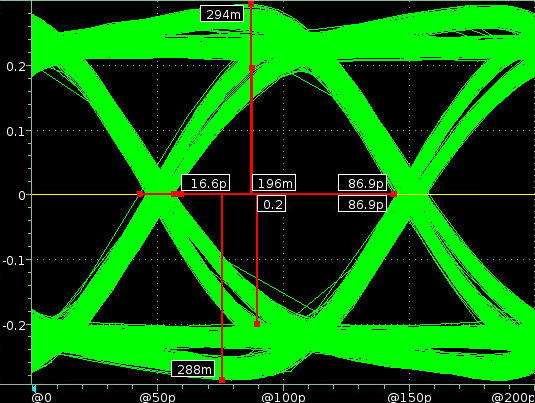
\includegraphics[width=\linewidth]{chapter4/post_ext/eyes/EQ3/EQ3_FF_Rmax.png}
	\caption{Res\_max}
\end{subfigure}
\caption{Post extraction EQ3 eye diagrams for resistor corners at \ac{FF}}\label{fig:eye_EQ3_FF_pext}
\end{figure}

\begin{table}[H]
 \centering
 \caption{Post extraction EQ3 \ac{RX} eye diagram metrics across resistor corners at \ac{FF}}
 \label{tab:eq3_eye_FF_pext}
 \begin{tabular}{ccc}
  \hline \hline
  \textbf{Corner} & \textbf{Height} & \textbf{Width} \\
  \hline
  Res\_min & \SI{359}{\milli\volt} & \SI{86.9}{\pico\second} \\
  Res\_nom & \SI{386}{\milli\volt} & \SI{86.4}{\pico\second} \\
  Res\_max & \SI{396}{\milli\volt} & \SI{86.9}{\pico\second} \\
  \hline \hline
 \end{tabular}
\end{table}


The corresponding post-extraction EQ3 eye diagrams at \ac{SS} are shown in Figure~\ref{fig:eye_EQ3_SS_pext}.

\begin{figure}[H]
\centering
\begin{subfigure}{0.4\textwidth}
	\centering
	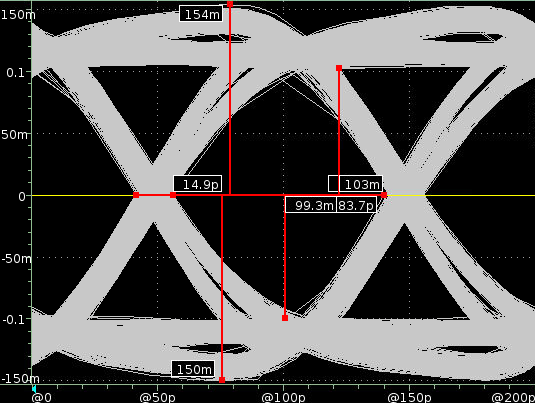
\includegraphics[width=\linewidth]{chapter4/post_ext/eyes/EQ3/EQ3_SS_Rmin.png}
	\caption{Res\_min}
\end{subfigure}
\begin{subfigure}{0.4\textwidth}
	\centering
	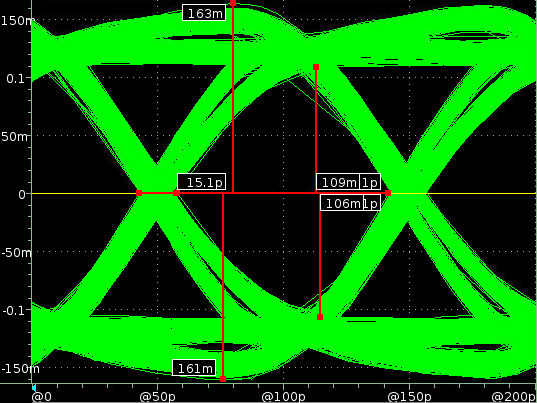
\includegraphics[width=\linewidth]{chapter4/post_ext/eyes/EQ3/EQ3_SS_Rnom.png}
	\caption{Res\_nom}
\end{subfigure}
\begin{subfigure}{0.4\textwidth}
	\centering
	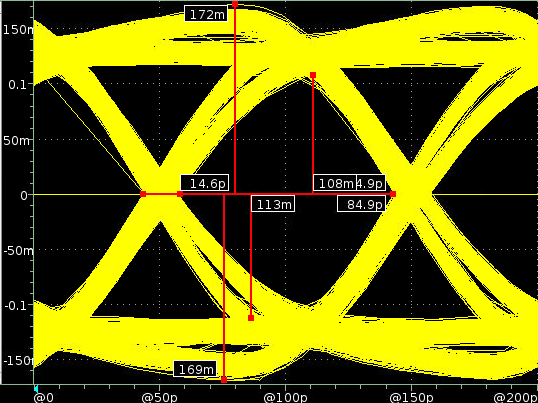
\includegraphics[width=\linewidth]{chapter4/post_ext/eyes/EQ3/EQ3_SS_Rmax.png}
	\caption{Res\_max}
\end{subfigure}
\caption{Post extraction EQ3 eye diagrams for resistor corners at \ac{SS}}\label{fig:eye_EQ3_SS_pext}
\end{figure}

\begin{table}[H]
 \centering
 \caption{Post extraction EQ3 \ac{RX} eye diagram metrics across resistor corners at \ac{SS}}
 \label{tab:eq3_eye_SS_pext}
 \begin{tabular}{ccc}
  \hline \hline
  \textbf{Corner} & \textbf{Height} & \textbf{Width} \\
  \hline
  Res\_min & \SI{202.3}{\milli\volt} & \SI{83.7}{\pico\second} \\
  Res\_nom & \SI{215}{\milli\volt} 	 & \SI{83.1}{\pico\second} \\
  Res\_max & \SI{221}{\milli\volt} 	 & \SI{84.9}{\pico\second} \\
  \hline \hline
 \end{tabular}
\end{table}



These results indicate that, for the evaluated EQ3 configuration, resistor variation has a stronger influence on the vertical eye opening than on the horizontal timing opening. The larger difference between the \ac{FF} and \ac{SS} eye heights further shows that transistor-level \ac{PVT} variation has a more pronounced effect on received voltage margin than the resistor-corner variation within a given \ac{PVT} condition.

\section{Pre and Post Extraction Comparison}\label{sec:pre_post_comparison}

Table~\ref{tab:pre_post_summary} compares the principal pre- and post-extraction results for the representative EQ3 configuration at the \ac{TT} corner. EQ3 is retained as the reference case because it provides the largest pre-extraction \ac{RX} eye and remains one of the two strongest post-extraction equalization configurations. For consistency, the \ac{DE} values in this comparison are reported as positive magnitudes.


\begin{table}[htbp]
 \centering
 \caption{Pre- versus post-extraction results at the \ac{TT} corner (EQ3, unless noted)}
 \label{tab:pre_post_summary}
 \begin{tabular}{lccc}
  \hline \hline
  \textbf{Metric} & \textbf{Pre-extraction} & \textbf{Post-extraction} & \textbf{$\Delta$} \\
  \hline
  \ac{PS} [dB]
  & 3.01 & 3.121 & $+3.7\%$ \\

  \ac{DE} magnitude [dB]
  & 6.63 & 6.114 & $-7.8\%$ \\

  Output rise time [ps]
  & 27.3 & 42.1 & +54.2\% \\

  Output fall time [ps]
  & 22.8 & 35.6 & +56.1\% \\

  \ac{RX} eye height [mV]
  & 231 & 322 & $+39.4\%$ \\

  \ac{RX} eye width [ps]
  & 79.6 & 84.7 & $+6.4\%$ \\

  \ac{RX} crossover width [ps]
  & 45.1 & 15.6 & $-65.4\%$ \\

  $Z_{out,diff}$, \#$en_{nom}$ (Res\_nom)
  & 15 & 19 & $+26.7\%$ \\

  Power consumption [mW] (Res\_nom)
  & 25.5 & 24.42 & $-4.2\%$ \\
  \hline \hline
 \end{tabular}
\end{table}

The comparison shows that parasitic extraction significantly modifies the transmitter behaviour, but that the effect is not a uniform degradation of all metrics. The clearest direct penalty is observed in the output transition times. At \ac{TT}, the rise time increases from 27.3~ps to 42.1~ps, while the fall time increases from 22.8~ps to 35.6~ps, corresponding to increases of approximately 54.2\% and 56.1\%, respectively. The similar relative degradation of the two transitions indicates that parasitic extraction introduces an overall increase in the effective time constants of the high-speed output paths, expected with the increase that the parasitics introduces to the RC time constant, $\tau$, of the nets. The rise--fall asymmetry already present before extraction remains.

The equalization coefficients are also modified after extraction. For EQ3 at \ac{TT}, the \ac{PS} changes from \SI{3.01}{\decibel} to \SI{3.121}{\decibel}, while the \ac{DE} magnitude decreases from \SI{6.63}{\decibel} to \SI{6.114}{\decibel}. More generally, Table~\ref{tab:PVT_eq_results_pext_deviation} shows that the effect becomes much stronger for \ac{DE} at the \ac{SS} corner. Together with the EQ1 retuning results, this demonstrates that extraction alters the effective relative weighting of the tap currents and that the optimum enable mapping can become corner-dependent. The available results do not, however, isolate this behaviour to one individual tap current alone.

The termination network is similarly affected by the physical implementation. For \ac{TT} and Res\_nom, the enable count associated with the nominal output impedance changes from 15 before extraction to 19 after extraction. The programmable termination bank therefore provides useful margin for compensating not only resistor-process variation but also the additional resistance introduced by the extracted interconnect.

Despite the slower transmitter transitions, the received EQ3 eye does not degrade. The \ac{RX} eye height increases from \SI{231}{\milli\volt} to \SI{322}{\milli\volt}, while the eye width increases from \SI{79.6}{\pico\second} to \SI{84.7}{\pico\second}. At the same time, the measured crossover width decreases substantially, from \SI{45.1}{\pico\second} before extraction to \SI{15.6}{\pico\second} after extraction, corresponding to a reduction of approximately 65.4\%.

A similar behaviour is observed for EQ4, whose crossover width decreases from \SI{49.7}{\pico\second} before extraction to \SI{16.0}{\pico\second} after extraction, a reduction of approximately 67.8\%. The post-extraction EQ3 crossover is also relatively insensitive to the evaluated process corner, varying from \SI{15.1}{\pico\second} at \ac{SS} to \SI{16.9}{\pico\second} at \ac{FF}.

The substantial reduction in crossover width indicates a more concentrated distribution of the received transition crossings in the extracted simulations. However, this observation should not be interpreted as a direct measurement of \ac{DJ} or total jitter, since the normative jitter decomposition was not performed. Furthermore, because extraction modifies several circuit properties simultaneously, including the transition times, effective tap weighting, and termination operating point, the reduction cannot be uniquely attributed to a single parasitic mechanism.

Finally, the EQ3 power consumption at \ac{TT}, Res\_nom changes only moderately, from \SI{25.5}{\milli\watt} before extraction to \SI{24.42}{\milli\watt} after extraction. This \SI{4.2}{\percent} difference is small compared with the changes observed in transition time and equalization accuracy and does not materially alter the power-performance conclusions of the design.

\subsection{Evaluation Against USB 3.2 Gen 2 Electrical Requirements}\label{sec:usb32_compliance}

Table~\ref{tab:usb32_compliance} summarizes the principal simulated transmitter metrics against the corresponding \ac{USB} 3.2 Gen~2 electrical limits. The post-extraction values correspond to the latest results presented in this chapter. Where programmability is required to obtain a compliant operating point, this is explicitly indicated.


\begin{threeparttable}
\centering
\small
\caption{Summary of the evaluated USB 3.2 Gen 2 transmitter electrical requirements, pre- versus post-extraction}
\label{tab:usb32_compliance}

\begin{tabular}{p{3.2cm}p{2.8cm}p{2.3cm}p{2.3cm}p{2.8cm}}
\hline \hline

\textbf{Requirement} &
\textbf{\ac{USB} 3.2 Specification} &
\textbf{Pre-extraction} &
\textbf{Post-extraction} &
\textbf{Status} \\

\hline

Unit Interval &
\SIrange{99.97}{100.03}{\pico\second} &
\SI{100}{\pico\second} &
\SI{100}{\pico\second} &
Compliant \\

\hline

Differential output voltage swing (EQ0) &
\SIrange{0.8}{1.2}{\volt_{pp}} &
\SI{1.17}{\volt_{pp}} (\ac{TT}) &
\SI{1.10}{\volt_{pp}} (\ac{TT}) &
Compliant \\

\hline

\ac{DC} differential output impedance &
\SIrange{72}{120}{\ohm} &
Compliant code available &
Compliant code available &
Compliant with corner-specific code$^{[1]}$ \\

\hline

Preshoot (EQ3, \ac{TT}) &
\SIrange{1.2}{3.2}{\decibel} &
\SI{3.01}{\decibel} &
\SI{3.121}{\decibel} &
Compliant \\

\hline

De-emphasis magnitude (EQ3, \ac{TT}) &
\SIrange{2.1}{7}{\decibel} &
\SI{6.63}{\decibel} &
\SI{6.114}{\decibel} &
Compliant \\

\hline

Eye diagram height (EQ3, \ac{TT}, \ac{RX}) &
\SIrange{70}{1200}{\milli\volt} &
\SI{231}{\milli\volt} &
\SI{322}{\milli\volt} &
Within numerical limit; normative eye procedure not fully evaluated \\

\hline \hline
\end{tabular}

\begin{tablenotes}

\item[1] \footnotesize{The complete \SIrange{72}{120}{\ohm} interval is not
available for every combined \ac{PVT} and resistor corner. However, at least one
termination-bank configuration within the normative range is available for every
evaluated corner.}
\end{tablenotes}
\end{threeparttable}

\vspace*{10px}

The results in Table~\ref{tab:usb32_compliance} demonstrate that the simulated transmitter provides sufficient programmable range to obtain operating points within the evaluated \ac{USB} 3.2 Gen~2 numerical limits for output swing, equalization, and output impedance after parasitic extraction. The simulated EQ3 receiver eye height also lies within the numerical eye-height range defined by the standard, although the complete normative transmitter-eye measurement procedure was not reproduced. The EQ1 tuning study further shows, however, that the required equalization code can depend on \ac{PVT}, rather than being represented by one universal post-layout mapping.

These results should not be interpreted as a complete transmitter compliance demonstration. In particular, the normative \ac{TX}-eye and jitter methodology defined by the \ac{USB} 3.2 specification was not reproduced in full. This methodology includes the prescribed Gen~2 compliance patterns, reference channel, compliance receiver equalization and jitter-transfer processing, measurement over $10^6$ consecutive \ac{UI}, and extrapolation of the jitter results to a BER of $10^{-12}$. Furthermore, not all normative transmitter electrical parameters were evaluated in the present work. The results presented here therefore demonstrate agreement with the relevant numerical limits for the evaluated simulated metrics and sufficient post-layout tuning range, rather than formal \ac{USB-IF} compliance.

\section{Comparison with the State of the Art}
\label{sec:sota_comparison}

The results presented in the previous sections establish the post-layout performance of the proposed transmitter against the \ac{USB}~3.2 Gen~2 electrical requirements. To place these results in a broader context, Table~\ref{tab:sota_comparison} compares the implemented driver with representative \ac{CML} and \ac{CML}-based transmitters operating at similar data rates.

A direct numerical ranking is not appropriate because the reported circuits target different applications, channel conditions, voltage swings, circuit boundaries, and verification methodologies. In particular, some publications report fabricated-silicon measurements whereas the results of the present work are obtained from post-layout extracted simulations. The comparison is therefore intended primarily to identify architectural and performance trade-offs rather than to claim superiority based on a single figure of merit.

\begin{table}[!ht]
    \centering
    \caption{Comparison with representative \ac{CML} and \ac{CML}-based high-speed transmitters.}
    \label{tab:sota_comparison}
    \resizebox{\textwidth}{!}{%
    \begin{tabular}{lcccccccc}
        \hline
		\hline
        \textbf{Work} &
        \textbf{Tech.} &
        \textbf{Rate} &
        \textbf{Equalization} &
        \textbf{Supply} &
        \textbf{Channel / loss} &
        \textbf{Eye / swing} &
        \textbf{Consumption} &
        \textbf{Verification} \\
        \hline

        Rylyakov and Rylov
        \cite{rylyakov2005} &
        90 nm &
        10 Gb/s &
        4-tap FFE &
        1.2/1.65 V &
        16-in backplane &
        0.9 Vppd &
        174 mW &
        Silicon \\

        Weiss \textit{et al.}
        \cite{weiss2006} &
        130 nm &
        10 Gb/s &
        3-tap FIR &
        1.5 V &
        24.3 dB @ 4.5 GHz$^{a}$ &
        BER $<10^{-12}$ &
        -- &
        Silicon \\

        Chen \textit{et al.}
        \cite{chen_switchable_cml_2016} &
        130 nm &
        10 Gb/s &
        -- &
        3.3 V &
        Microstrip model &
        1.6 Vppd &
        10 mA &
        Post-layout sim. \\

        Yi \textit{et al.}
        \cite{yi2016} &
        65 nm &
        9 Gb/s &
        VM pre-emphasis + CML &
        1.0 V &
        12-in FR-4 &
        40 mVppd &
        2.8 mW TX &
        Silicon \\

        Lv and Zhang
        \cite{lv_cml_28nm_2018} &
        28 nm &
        12.5 Gb/s &
        Current pre-emphasis &
        1.05 V &
        -- &
        604 mVppd &
        28.9 mW &
        Post-layout sim. \\

        Choi \textit{et al.}
        \cite{choi2019} &
        55 nm &
        10 Gb/s &
        2-tap + cap. peaking &
        1.2 V &
        12.3 dB @ 5 GHz &
        160 mV / 0.92 UI$^{b}$ &
        36.25 mA$^{c}$ &
        Post-layout sim. \\

        \textbf{This work} &
        \textbf{55 nm} &
        \textbf{10 Gb/s} &
        \textbf{3-tap FFE} &
        \textbf{1.2 V} &
        \textbf{21.6 dB @ 5 GHz} &
        \textbf{322 mV / 0.847 UI$^{d}$} &
        \textbf{24.42 mW} &
        \textbf{Post-layout sim.} \\

        \hline
		\hline
    \end{tabular}}
    
    \vspace{1mm}
    \begin{minipage}{0.98\textwidth}
        \footnotesize
        $^{a}$ Motherboard-channel attenuation reported at the
        \SI{4.5}{\giga\hertz} Nyquist frequency for the
        9 Gbps experiment. \\
        $^{b}$ Differential received eye height and normalized eye width
        reported after the \SI{12.3}{\decibel} channel. \\
        $^{c}$ Includes the pre-driver and timing circuitry and is therefore
        not directly comparable with power numbers whose circuit boundaries
        differ. \\
        $^{d}$ EQ3 post-extraction receiver eye. The
        \SI{84.7}{\pico\second} eye width corresponds to 0.847~UI at
        10 Gbps.
    \end{minipage}
\end{table}

The most direct architectural comparison is with the work of Weiss \textit{et al.} \cite{weiss2006}, since both transmitters employ current-domain multi-tap \ac{FIR} equalization around 10 Gbps. Their implementation demonstrates experimentally that summing independently weighted \ac{CML} tap currents is effective for compensating strongly attenuating electrical channels. The present design follows the same general current-domain equalization principle but uses explicit pre-cursor, main-cursor, and post-cursor segmentation derived from the \ac{USB} preshoot and de-emphasis requirements. In addition, both the tap-current sources and output termination are digitally segmented to provide adjustment after physical implementation. The principal advantage of the earlier work is its experimental validation, including direct \ac{BER} measurements, which is not available for the present design.

The four-tap transmitter of Rylyakov and Rylov \cite{rylyakov2005} provides another useful comparison because it also combines programmable current weighting with a \ac{CML} output stage. At 10 Gbps, that implementation reports \SI{174}{\milli\watt} total transmitter consumption under its \SI{125}{\celsius} test condition. The substantially lower numerical power of the present transmitter, \SI{24.42}{\milli\watt} at the nominal condition, reflects in part the benefits of a more scaled technology and a different circuit boundary and supply arrangement. It should therefore not be interpreted as a technology-normalized power improvement. Nevertheless, it shows that a programmable multi-tap current-mode architecture can be implemented at 10 Gbps with a power consumption in the tens-of-milliwatt range while retaining a large programmable output swing.

The work of Lv and Zhang \cite{lv_cml_28nm_2018} is closer in terms of simulated power. Their \SI{28}{\nano\meter}, 12.5 Gbps driver consumes \SI{28.9}{\milli\watt}, compared with \SI{24.42}{\milli\watt} for EQ3 in the present implementation. This corresponds to approximately \SI{2.31}{\pico\joule\per\bit} for their reported operating point and \SI{2.44}{\pico\joule\per\bit} for the present design. These figures are of the same order despite the different technology nodes and output requirements. However, the comparison remains approximate because the two circuits employ different equalization structures, output swings, and channel environments.

The implementation by Choi \textit{et al.} \cite{choi2019} provides the closest technology-level comparison. Both designs operate at 10 Gbps in \SI{55}{\nano\meter} \ac{CMOS} from a \SI{1.2}{\volt} supply. Choi \textit{et al.} use two current-mode taps together with reconfigurable capacitive peaking to reduce the static-current penalty associated with stronger equalization. Their post-layout simulations produce a \SI{160}{\milli\volt} eye height and a 0.92~UI eye width after a channel with \SI{12.3}{\decibel} insertion loss at \SI{5}{\giga\hertz}. In comparison, the present EQ3 configuration produces a \SI{322}{\milli\volt} receiver eye height and a \SI{84.7}{\pico\second}, or 0.847~UI, eye width after the \ac{USB-IF} reference channel, whose insertion loss is \SI{21.6}{\decibel} at the same Nyquist frequency. The larger channel loss in the present verification makes a direct eye-opening comparison inappropriate, but it demonstrates that the three-tap programmable structure retains substantial voltage and timing margin under the more strongly attenuating reference channel used in this work.

The Choi implementation draws \SI{36.25}{\milli\ampere} from the \SI{1.2}{\volt} supply when the pre-driver and timing circuits are included, corresponding to approximately \SI{43.5}{\milli\watt}. Although this value is numerically higher than the \SI{24.42}{\milli\watt} reported for EQ3 in the present transmitter, the circuit boundaries are not equivalent. The difference should therefore not be interpreted as a direct power-efficiency advantage. Instead, the two implementations illustrate different strategies: capacitive peaking reduces the current required for additional high-frequency boost, whereas the present architecture uses digitally controllable current-domain taps to maximize configurability and to implement the required \ac{USB} preshoot and de-emphasis presets directly.

The transmitter of Yi \textit{et al.} \cite{yi2016} demonstrates the opposite end of the power--swing trade-off. Its measured transmitter consumes only \SI{2.8}{\milli\watt} at 9 Gbps, substantially below the present design. However, this result is obtained with only \SI{40}{\milli\volt} peak-to-peak differential channel swing, no conventional \ac{TX}-end termination, and a receiver specifically designed for an input sensitivity of approximately \SI{9}{\milli\volt}. Its voltage-mode pre-emphasis path also eliminates the low-frequency de-emphasis current of a conventional current-mode equalizer. The result therefore demonstrates that substantially higher energy efficiency is possible when the transmitter and receiver are co-designed for very-low-swing signaling, but it does not represent a directly equivalent solution to the \ac{USB} transmitter requirements addressed here.

The main distinction of the present work is consequently not a record absolute power or data rate. Instead, it is the combination of a conventional current-steering output structure with three independently programmable \ac{FFE} taps, programmable termination, and an explicit post-layout investigation across transistor and resistor process corners. The extracted results show why this configurability is important. At the representative EQ3 operating point, extraction changes the rise and fall times from \SI{27.3}{\pico\second} and \SI{22.8}{\pico\second} to \SI{42.1}{\pico\second} and \SI{35.6}{\pico\second}, respectively, and changes the termination-bank setting required to obtain the nominal differential output impedance. The equalization mapping also becomes \ac{PVT}-dependent for some presets. These effects would not be visible from a nominal schematic-only comparison.

From this perspective, the principal contribution of the proposed architecture is its ability to recover specification-compatible operating points after the physical implementation modifies the nominal circuit behaviour. The segmented current banks provide sufficient range to retune equalization, while the segmented termination network provides corresponding impedance adjustment. This flexibility is particularly relevant for an interface such as \ac{USB}~3.2 Gen~2, for which output swing, preshoot, de-emphasis, and output impedance must be simultaneously controlled.

The comparison must nevertheless be qualified by the verification status. Rylyakov and Rylov, Weiss \textit{et al.}, and Yi \textit{et al.} report measurements from fabricated silicon, including \ac{BER} measurements in the first two cases. In contrast, the present work is verified at schematic and post-extraction simulation levels. Consequently, the results demonstrate the performance and programmability of the implemented layout but do not yet establish measured silicon performance. Package parasitics, fabrication mismatch, laboratory measurement uncertainty, and the complete normative \ac{DJ}, \ac{RJ}, \ac{TJ}, and \ac{BER} characterization remain to be evaluated experimentally.